\begin{enumerate}[label=\thesection.\arabic*,ref=\thesection.\theenumi]
\numberwithin{equation}{enumi}
\numberwithin{figure}{enumi}
\numberwithin{table}{enumi}
\item 
\label{chapters/12/8/3/1}
%\documentclass[journal,12pt,twocolumn]{IEEEtran}
\usepackage{graphicx}
\usepackage{listings}
\usepackage[utf8]{inputenc}
\usepackage{caption}
\usepackage{hyperref}
\usepackage[cmex10]{amsmath}
\usepackage{array}
\usepackage{gensymb}
\usepackage{booktabs}
\usepackage{etoolbox}
\usepackage{amssymb}
\patchcmd{\section}{\centering}{}{}{}
\providecommand{\norm}[1]{\left\lVert#1\right\rVert}
\providecommand{\abs}[1]{\left\vert#1\right\vert}
\let\vec\mathbf

\makeatletter
\newcommand\xleftrightarrow[2][]{%
  \ext@arrow 9999{\longleftrightarrowfill@}{#1}{#2}}
\newcommand\longleftrightarrowfill@{%
  \arrowfill@\leftarrow\relbar\rightarrow}
\makeatother
\title{Matrix Problems \textbf{\\Conics }}
\author{Manoj Chavva} 
\newcommand{\myvec}[1]{\ensuremath{\begin{pmatrix}#1\end{pmatrix}}}
\newcommand{\mydet}[1]{\ensuremath{\begin{vmatrix}#1\end{vmatrix}}}
\providecommand{\brak}[1]{\ensuremath{\left(#1\right)}}
\providecommand{\lbrak}[1]{\ensuremath{\left(#1\right.}}
\providecommand{\rbrak}[1]{\ensuremath{\left.#1\right)}}
\providecommand{\sbrak}[1]{\ensuremath{{}\left[#1\right]}}

\begin{document}
\maketitle
\section{Problem Statement}

\noindent Smaller area enclosed by the circle $x^2 + y^2 = 4$ and the line $x + y = 2$. 
\begin{enumerate}
\item $2(\pi -2)$
\item $\pi -2$
\item $2\pi -1$
\item $2(\pi +2)$
\end{enumerate}


\begin{figure}[h]
\includegraphics[width=1\columnwidth]{./figs/conic.png}
\caption{Smaller region between Circle and Line}
\label{fig:conic}
\end{figure}

\raggedright \textbf{Given}: \\
Equation of circle is  
\begin{equation} x^2 + y^2 = 4
\end{equation}
Equation of line is 
\begin{equation}
x+y=2
\end{equation}
\textbf{To Find:} \\
To find the intersection points and area of shaded region shown in figure\
\section{Construction}

\begin{table}[h!]
\begin{center}
\setlength{\arrayrulewidth}{0.5mm}
\renewcommand{\arraystretch}{1.5}
    \begin{tabular}{|l|c|}
    \hline 
    \textbf{Points} & \textbf{coordinates} \\ \hline
   $\vec{A}$ & $\myvec{
   0\\
   2
   } $ \\\hline
   $\vec{B}$ & $\myvec{
   2\\
   0
   } $ \\\hline
      \end{tabular}
  \end{center}
\end{table}
\newpage
\section{solution}
The given circle can be expressed as conics with parameters,
\begin{equation}
\vec{V}=\myvec{
4 & 0\\
0 & 4
}
\end{equation}
\begin{equation}
\vec{u}=0 
\end{equation}
\begin{equation}
f=-16
\end{equation}

The given line equation can be written as\\ 
\begin{align} 
	\vec{x}=\begin{pmatrix}2 \\ 0 \\ \end{pmatrix}+k\begin{pmatrix}\frac{1}{2} \\ -\frac{1}{2} \\ \end{pmatrix}
\end{align}
The points of intersection of the line, \\ 
\begin{equation}
L: \quad \vec{x} = \vec{q} + \kappa \vec{m} \quad \kappa \in \mathbb{R}
\end{equation}

with the conic section, \\ 
\begin{align}
	\vec{x}^{\top}\vec{V}\vec{x} + 2\vec{u}^{\top} \vec{x} + f = 0
\end{align}
are given by \\
\begin{align}
\vec{x}_i = \vec{q} + \kappa_i \vec{m}
\end{align}
where, \\

\begin{equation*}
\kappa_i = \frac{1}
{
\vec{m}^T\vec{V}\vec{m}
}
\lbrak{-\vec{m}^T\brak{\vec{V}\vec{q}+\vec{u}}}
\pm
\end{equation*}
\begin{equation}
\rbrak{\sqrt{
\sbrak{
\vec{m}^T\brak{\vec{V}\vec{q}+\vec{u}}
}^2
-
\brak
{
\vec{q}^T\vec{V}\vec{q} + 2\vec{u}^T\vec{q} +f
}
\brak{\vec{m}^T\vec{V}\vec{m}}
}
}
\end{equation}
On substituting\\
\begin{align}
\vec{q} &= \myvec{
2\\
0
} 
\end{align}
\begin{align}
\vec{m} = \myvec{\frac{1}{2} \\ -\frac{1}{2}}
\end{align}
With the given as in eq(3),(4),(5),\\ 

The value of $\kappa$ ,\\
\begin{equation}
\kappa =0,-4
\end{equation}
    
By substituting eq(13) in eq(6) we get the
points of intersection of line with circle \\
\begin{align}
    \vec{A}=\myvec{
0\\
2
    }
\end{align}
\begin{align}
    \vec{B}=\myvec{
2\\
0
    }
\end{align}
From the figure \\
Total area of portion is given by,\\ 
Total Area=(area of circle in first quadrant)-(area of a triangle \textbf{AOB})

\subsection*{Area of triangle}

\begin{align}
\implies A_1=\int_{0}^{2} (2-x) \,dx
\end{align}
By solving the above equation we get area of triangle as 2 units
\subsection*{Area of circle}

\begin{align} 
\implies A_2=\int_{0}^{2}\sqrt{4-x^2} \,dx 
\end{align}
By solving the above equation we get area of circle $\pi$

The total area is
$\implies \vec{A}=\pi - 2$


\begin{table}[h]
\large
\begin{tabular}{lll}
\multicolumn{3}{l}{Get Python Code for image from}                                                 \\ \hline
\multicolumn{3}{|l|}{\url{https://github.com/ManojChavva/FWC/blob/main/Matrix/conics/code/conic.py}} \\ 
 \hline
\multicolumn{3}{l}{Get LaTex code from}                                                            \\ \hline
\multicolumn{3}{|l|}{\url{https://github.com/ManojChavva/FWC/blob/main/Matrix/conics/conic.tex}}            \\ \hline
\end{tabular}
\end{table}



\end{document}





\item 
\label{chapters/12/8/3/2}
\iffalse
\documentclass[10pt,a4paper]{report}
\usepackage[latin1]{inputenc}
\usepackage{amsmath}
\usepackage{amsfonts}
\usepackage{amssymb}
\usepackage{graphicx}
\usepackage{hyperref}
\usepackage{multicol}
\usepackage[margin=0.5in]{geometry}
\usepackage{tikz}
\usepackage[document]{ragged2e}
\usepackage{romannum}
\usetikzlibrary{arrows,shapes.gates.logic.US,shapes.gates.logic.IEC,calc}
\usepackage{titlesec}
\titlespacing{\subsection}{1pt}{\parskip}{3pt}
\titlespacing{\subsubsection}{0pt}{\parskip}{-\parskip}
\titlespacing{\paragraph}{0pt}{\parskip}{\parskip}
\newcommand{\myvec}[1]{\ensuremath{\begin{pmatrix}#1\end{pmatrix}}}
\let\vec\mathbf

\newcommand{\mydet}[1]{\ensuremath{\begin{vmatrix}#1\end{vmatrix}}}
\providecommand{\brak}[1]{\ensuremath{\left(#1\right)}}
\providecommand{\lbrak}[1]{\ensuremath{\left(#1\right.}}
\providecommand{\rbrak}[1]{\ensuremath{\left.#1\right)}}
\providecommand{\sbrak}[1]{\ensuremath{{}\left[#1\right]}}

\begin{document}

\begin{multicols}{2}
\raggedright {\includegraphics[scale=0.06]{iith_logo.png}} \vspace{3mm}\\ \raggedleft Hari Venkateswarlu Annam\vspace{2mm}\\ 
\raggedleft  FWC22058\vspace{2mm}\\ 
\raggedleft hariannam99@gmail.com \vspace{2mm}\\ 
\raggedleft Oct 2022 \vspace{5mm}\\
\end{multicols}

\centering \Large \textbf{MATRIX : CONIC ASSIGNMENT} \normalsize \vspace{10mm}

\begin{multicols}{2}

\section{Problem:}  
\fi
Find the area between the curves $y=x$ and $y=x^2$.
\\
\solution
	\begin{figure}[!h]
		\centering
 \includegraphics[width=\columnwidth]{chapters/12/8/3/2/figs/figure.png}
		\caption{}
		\label{fig:12/8/3/2}
  	\end{figure}
\iffalse
\section{Solution: }
\raggedright \textbf{Input Parameters :}\\ \vspace{2mm}
\centering Curve Equation : $y=x^2$. \\ \vspace{1mm}
Line Equation : $y=x$.\\
\vspace{3mm}

\raggedright \textbf{To Find :}\\ \vspace{2mm}
\begin{enumerate}
\item Comparing the given curve equation with the standard equation of the conics and finding it's parameters.
\item Finding the required parameters for the line equation.
\item Finding the Point of Intersection of the to the curve.
\item Finding the area between the curve.
\end{enumerate}

\raggedright \textbf{Step - 1 :}\\ \vspace{2mm}
Curve Equation : $y=x^2$. \\ \vspace{1mm}
The standard equation of the conics is given as :
\begin{align}
\vec{x}^{\top}\vec{V}\vec{x}+2\vec{u}^{\top}\vec{x}+f=0
\end{align}
\fi
The given curve  can be expressed as a conic with parameters
\begin{align}
	\vec{V} &= \myvec{1 & 0\\0 & 0}, \vec{u} = \myvec{0 \\-\frac{1}{2}}, f = 0
	\end{align}
\iffalse
\raggedright \textbf{Step - 2 :}\\ \vspace{2mm}
Line Equation : $y=x$. \\ \vspace{1mm}
From the above line equation below vectors are taken
\fi
The given line parameters are
\begin{align}
\vec{h} = \myvec{0 \\0}, \vec{m}=\myvec{1\\1}
\end{align}
\iffalse

\raggedright \textbf{Step - 3 :}\\ \vspace{2mm}
The points of intersection of the line, \\ 
\begin{align}
L: \quad \vec{x} = \vec{q} + \mu \vec{m} \quad \mu \in \mathbb{R}
\end{align}
with the conic section, \\ 
\begin{align}
	\vec{x}^{\top}\vec{V}\vec{x} + 2\vec{u}^{\top} \vec{x} + f = 0
\end{align}
are given by \\
\begin{align}
\vec{x}_i = \vec{q} + \mu_i \vec{m}
\end{align}
where, \\
{\tiny
\begin{multline}
\mu_i = \frac{1}
{
\vec{m}^T\vec{V}\vec{m}
}
\lbrak{-\vec{m}^T\brak{\vec{V}\vec{q}+\vec{u}}}
\\
\pm
\rbrak{\sqrt{
\sbrak{
\vec{m}^T\brak{\vec{V}\vec{q}+\vec{u}}
}^2
-
\brak
{
\vec{q}^T\vec{V}\vec{q} + 2\vec{u}^T\vec{q} +f
}
\brak{\vec{m}^T\vec{V}\vec{m}}
}
}
\end{multline}
}
\raggedright On substituting $\vec{V},\vec{q} ,\vec{m}$ in the above equation,
we get the values of $\mu$. By substituting the values of $\mu$ in eq(6), \\we get the points of intersection of line with the given curve. \\
\centering $i.e., \vec{x_1},\vec{x_2}$\\ 
\fi
Substituting the given parameters in 
\eqref{eq:tangent_roots},
\begin{align}
\vec{x_1}=\myvec{0\\0}, \vec{x_2}=\myvec{1\\1}.
\end{align}
From Fig. 
		\ref{fig:12/8/3/2},
the area bounded by the curve $y=x^2$ and line $y=x$ is given by
\begin{align}
	\int_{0}^{1} \brak{x 
	-\frac{x^2}{2}} \,dx = \frac{1}{6}
\end{align}
\iffalse

\centering By solving we get the required area\\
$\therefore A = \frac{1}{6}$ 



\section{Termux Commands :}
\centering bash rncom.sh ..... Using Shell commands.


\section{Plot :} 
\begin{center}
  \includegraphics[scale=0.55]{figure.png}
  	\end{center}

 
\end{multicols}
\end{document}
\fi

\item 
\label{chapters/12/8/3/3}
\iffalse
\documentclass[journal,10pt,twocolumn]{article}
\usepackage{graphicx}
\usepackage[margin=0.5in]{geometry}
\usepackage[cmex10]{amsmath}
\usepackage{array}
\usepackage{booktabs}
\usepackage{mathtools}
\title{\textbf{Conic section Assignment}}
\author{Jyothsna Paluchuri}
\date{September 2022}


\providecommand{\norm}[1]{\left\lVert#1\right\rVert}
\providecommand{\abs}[1]{\left\vert#1\right\vert}
\let\vec\mathbf
\newcommand{\myvec}[1]{\ensuremath{\begin{pmatrix}#1\end{pmatrix}}}
\newcommand{\mydet}[1]{\ensuremath{\begin{vmatrix}#1\end{vmatrix}}}
\providecommand{\brak}[1]{\ensuremath{\left(#1\right)}}
\providecommand{\lbrak}[1]{\ensuremath{\left(#1\right.}}
\providecommand{\rbrak}[1]{\ensuremath{\left.#1\right)}}
\providecommand{\sbrak}[1]{\ensuremath{{}\left[#1\right]}}

\begin{document}

\maketitle
\paragraph{\textit{Problem Statement} -
\fi
Find the area of the region bounded by the curve $x^2=4y$ and the lines y=2 and y=4 and the y-axis in the first quadrant.
\\
\solution
	\begin{figure}[!h]
		\centering
 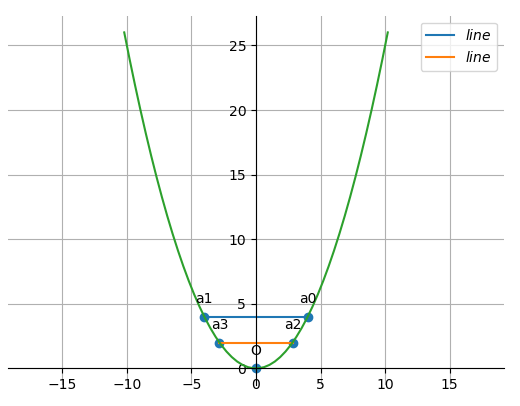
\includegraphics[width=\columnwidth]{chapters/12/8/3/3/figs/conic.png}
		\caption{}
		\label{fig:12/8/3/3}
  	\end{figure}
\iffalse

\section*{\large Solution}

\begin{figure}[h]
\centering
\includegraphics[width=1\columnwidth]{conic.png}

\caption{The parabola formed by the curve $x^2 = 4y$ and the lines y=2 and y=4}
\label{fig:parabola}
\end{figure}

The given equation of parabola $x^2 = 4y$ can be written in the general quadratic form as
\begin{align}
    \label{eq:conic_quad_form}
    \vec{x}^{\top}\vec{V}\vec{x}+2\vec{u}^{\top}\vec{x}+f=0
    \end{align}
where
\fi
The conic parameters are
\begin{align}
	\vec{V} = \myvec{1 & 0\\0 & 0},
	\vec{u} = \myvec{0\\-2},
	f = 0
	%\\
\end{align}
\iffalse
The point of intersection of the lines y=2 and y=4 to the parabola is given by



The points of intersection of the line 
\begin{align}
	L: \quad \vec{x} = \vec{q} + \mu \vec{m} \quad \mu \in \mathbf{R}
\label{eq:conic_tangent}
\end{align}
with the conic section are given by
\begin{align}
\vec{x}_i = \vec{q} + \mu_i \vec{m}
\label{eq:conic_tangent_pts}
\end{align}
%
where
{\tiny
\begin{multline}
\mu_i = \frac{1}
{
\vec{m}^T\vec{V}\vec{m}
}
\lbrak{-\vec{m}^T\brak{\vec{V}\vec{q}+\vec{u}}}
\\
\pm
\rbrak{\sqrt{
\sbrak{
\vec{m}^T\brak{\vec{V}\vec{q}+\vec{u}}
}^2
-
\brak
{
\vec{q}^T\vec{V}\vec{q} + 2\vec{u}^T\vec{q} +f
}
\brak{\vec{m}^T\vec{V}\vec{m}}
}
}
\label{eq:tangent_roots}
\end{multline}
}


\fi
The vector parameters of 
$y-4=0$
are
\begin{align}
	\vec{h}_1=\myvec{0\\4},
	\vec{m}_1=\myvec{1\\0}
\end{align}
Substituting the above in \eqref{eq:tangent_roots},
\begin{align}
\mu_i=4,-4
\end{align}
yielding
the points of intersection with the parabola as
\begin{align}
\vec{a}_0=\myvec{4\\4},
\vec{a}_1=\myvec{-4\\4}
\end{align}
Similarly, for 
the line $y-2=0$, the vector parameters are
\begin{align}
\vec{h}_2=\myvec{0\\2},
\vec{m}_2=\myvec{1\\0}
\end{align}
yielding 
\begin{align}
\mu_i=2.8,-2.8
\end{align}
and the points of intersection
\begin{align}
\vec{a}_2=\myvec{2.8\\2},
\vec{a}_3=\myvec{-2.8\\2}
\end{align}
From Fig.
		\ref{fig:12/8/3/3},
the area of the parabola between the lines $y=2$ and $y=4$ is given by
\begin{align}
\int_{0}^{4} \ 2\sqrt{y} \,dy-\int_{0}^{2} \ 2\sqrt{y} \,dy
=6.895 
\end{align}
\iffalse


\section*{\large Construction}

{
\setlength\extrarowheight{5pt}
\begin{tabular}{|l|c|}
    \hline 
    \textbf{Points} & \textbf{intersection points} \\ \hline
	a0 & $\myvec{
   -2.8\\
   2
   } $ \\\hline
	a1 & $\myvec{
   2.8\\
   2
   } $ \\\hline
    
	a3 & $\myvec{
   -4\\
   4
   } $ \\\hline
	a2 & $\myvec{
   4\\
   4
   } $ \\\hline
      
      \end{tabular}
}

\end{document}
\fi

\item 
\label{chapters/12/8/3/4}
%\documentclass[journal,12pt,twocolumn]{IEEEtran}
\usepackage{graphicx}
\usepackage{listings}
\usepackage[utf8]{inputenc}
\usepackage{caption}
\usepackage{hyperref}
\usepackage[cmex10]{amsmath}
\usepackage{array}
\usepackage{gensymb}
\usepackage{booktabs}
\usepackage{etoolbox}
\usepackage{amssymb}
\patchcmd{\section}{\centering}{}{}{}
\providecommand{\norm}[1]{\left\lVert#1\right\rVert}
\providecommand{\abs}[1]{\left\vert#1\right\vert}
\let\vec\mathbf

\makeatletter
\newcommand\xleftrightarrow[2][]{%
  \ext@arrow 9999{\longleftrightarrowfill@}{#1}{#2}}
\newcommand\longleftrightarrowfill@{%
  \arrowfill@\leftarrow\relbar\rightarrow}
\makeatother
\title{Matrix Problems \textbf{\\Conics }}
\author{Manoj Chavva} 
\newcommand{\myvec}[1]{\ensuremath{\begin{pmatrix}#1\end{pmatrix}}}
\newcommand{\mydet}[1]{\ensuremath{\begin{vmatrix}#1\end{vmatrix}}}
\providecommand{\brak}[1]{\ensuremath{\left(#1\right)}}
\providecommand{\lbrak}[1]{\ensuremath{\left(#1\right.}}
\providecommand{\rbrak}[1]{\ensuremath{\left.#1\right)}}
\providecommand{\sbrak}[1]{\ensuremath{{}\left[#1\right]}}

\begin{document}
\maketitle
\section{Problem Statement}

\noindent Smaller area enclosed by the circle $x^2 + y^2 = 4$ and the line $x + y = 2$. 
\begin{enumerate}
\item $2(\pi -2)$
\item $\pi -2$
\item $2\pi -1$
\item $2(\pi +2)$
\end{enumerate}


\begin{figure}[h]
\includegraphics[width=1\columnwidth]{./figs/conic.png}
\caption{Smaller region between Circle and Line}
\label{fig:conic}
\end{figure}

\raggedright \textbf{Given}: \\
Equation of circle is  
\begin{equation} x^2 + y^2 = 4
\end{equation}
Equation of line is 
\begin{equation}
x+y=2
\end{equation}
\textbf{To Find:} \\
To find the intersection points and area of shaded region shown in figure\
\section{Construction}

\begin{table}[h!]
\begin{center}
\setlength{\arrayrulewidth}{0.5mm}
\renewcommand{\arraystretch}{1.5}
    \begin{tabular}{|l|c|}
    \hline 
    \textbf{Points} & \textbf{coordinates} \\ \hline
   $\vec{A}$ & $\myvec{
   0\\
   2
   } $ \\\hline
   $\vec{B}$ & $\myvec{
   2\\
   0
   } $ \\\hline
      \end{tabular}
  \end{center}
\end{table}
\newpage
\section{solution}
The given circle can be expressed as conics with parameters,
\begin{equation}
\vec{V}=\myvec{
4 & 0\\
0 & 4
}
\end{equation}
\begin{equation}
\vec{u}=0 
\end{equation}
\begin{equation}
f=-16
\end{equation}

The given line equation can be written as\\ 
\begin{align} 
	\vec{x}=\begin{pmatrix}2 \\ 0 \\ \end{pmatrix}+k\begin{pmatrix}\frac{1}{2} \\ -\frac{1}{2} \\ \end{pmatrix}
\end{align}
The points of intersection of the line, \\ 
\begin{equation}
L: \quad \vec{x} = \vec{q} + \kappa \vec{m} \quad \kappa \in \mathbb{R}
\end{equation}

with the conic section, \\ 
\begin{align}
	\vec{x}^{\top}\vec{V}\vec{x} + 2\vec{u}^{\top} \vec{x} + f = 0
\end{align}
are given by \\
\begin{align}
\vec{x}_i = \vec{q} + \kappa_i \vec{m}
\end{align}
where, \\

\begin{equation*}
\kappa_i = \frac{1}
{
\vec{m}^T\vec{V}\vec{m}
}
\lbrak{-\vec{m}^T\brak{\vec{V}\vec{q}+\vec{u}}}
\pm
\end{equation*}
\begin{equation}
\rbrak{\sqrt{
\sbrak{
\vec{m}^T\brak{\vec{V}\vec{q}+\vec{u}}
}^2
-
\brak
{
\vec{q}^T\vec{V}\vec{q} + 2\vec{u}^T\vec{q} +f
}
\brak{\vec{m}^T\vec{V}\vec{m}}
}
}
\end{equation}
On substituting\\
\begin{align}
\vec{q} &= \myvec{
2\\
0
} 
\end{align}
\begin{align}
\vec{m} = \myvec{\frac{1}{2} \\ -\frac{1}{2}}
\end{align}
With the given as in eq(3),(4),(5),\\ 

The value of $\kappa$ ,\\
\begin{equation}
\kappa =0,-4
\end{equation}
    
By substituting eq(13) in eq(6) we get the
points of intersection of line with circle \\
\begin{align}
    \vec{A}=\myvec{
0\\
2
    }
\end{align}
\begin{align}
    \vec{B}=\myvec{
2\\
0
    }
\end{align}
From the figure \\
Total area of portion is given by,\\ 
Total Area=(area of circle in first quadrant)-(area of a triangle \textbf{AOB})

\subsection*{Area of triangle}

\begin{align}
\implies A_1=\int_{0}^{2} (2-x) \,dx
\end{align}
By solving the above equation we get area of triangle as 2 units
\subsection*{Area of circle}

\begin{align} 
\implies A_2=\int_{0}^{2}\sqrt{4-x^2} \,dx 
\end{align}
By solving the above equation we get area of circle $\pi$

The total area is
$\implies \vec{A}=\pi - 2$


\begin{table}[h]
\large
\begin{tabular}{lll}
\multicolumn{3}{l}{Get Python Code for image from}                                                 \\ \hline
\multicolumn{3}{|l|}{\url{https://github.com/ManojChavva/FWC/blob/main/Matrix/conics/code/conic.py}} \\ 
 \hline
\multicolumn{3}{l}{Get LaTex code from}                                                            \\ \hline
\multicolumn{3}{|l|}{\url{https://github.com/ManojChavva/FWC/blob/main/Matrix/conics/conic.tex}}            \\ \hline
\end{tabular}
\end{table}



\end{document}





\item 
\label{chapters/12/8/3/5}
%\documentclass[journal,12pt,twocolumn]{IEEEtran}
\usepackage{graphicx}
\usepackage{listings}
\usepackage[utf8]{inputenc}
\usepackage{caption}
\usepackage{hyperref}
\usepackage[cmex10]{amsmath}
\usepackage{array}
\usepackage{gensymb}
\usepackage{booktabs}
\usepackage{etoolbox}
\usepackage{amssymb}
\patchcmd{\section}{\centering}{}{}{}
\providecommand{\norm}[1]{\left\lVert#1\right\rVert}
\providecommand{\abs}[1]{\left\vert#1\right\vert}
\let\vec\mathbf

\makeatletter
\newcommand\xleftrightarrow[2][]{%
  \ext@arrow 9999{\longleftrightarrowfill@}{#1}{#2}}
\newcommand\longleftrightarrowfill@{%
  \arrowfill@\leftarrow\relbar\rightarrow}
\makeatother
\title{Matrix Problems \textbf{\\Conics }}
\author{Manoj Chavva} 
\newcommand{\myvec}[1]{\ensuremath{\begin{pmatrix}#1\end{pmatrix}}}
\newcommand{\mydet}[1]{\ensuremath{\begin{vmatrix}#1\end{vmatrix}}}
\providecommand{\brak}[1]{\ensuremath{\left(#1\right)}}
\providecommand{\lbrak}[1]{\ensuremath{\left(#1\right.}}
\providecommand{\rbrak}[1]{\ensuremath{\left.#1\right)}}
\providecommand{\sbrak}[1]{\ensuremath{{}\left[#1\right]}}

\begin{document}
\maketitle
\section{Problem Statement}

\noindent Smaller area enclosed by the circle $x^2 + y^2 = 4$ and the line $x + y = 2$. 
\begin{enumerate}
\item $2(\pi -2)$
\item $\pi -2$
\item $2\pi -1$
\item $2(\pi +2)$
\end{enumerate}


\begin{figure}[h]
\includegraphics[width=1\columnwidth]{./figs/conic.png}
\caption{Smaller region between Circle and Line}
\label{fig:conic}
\end{figure}

\raggedright \textbf{Given}: \\
Equation of circle is  
\begin{equation} x^2 + y^2 = 4
\end{equation}
Equation of line is 
\begin{equation}
x+y=2
\end{equation}
\textbf{To Find:} \\
To find the intersection points and area of shaded region shown in figure\
\section{Construction}

\begin{table}[h!]
\begin{center}
\setlength{\arrayrulewidth}{0.5mm}
\renewcommand{\arraystretch}{1.5}
    \begin{tabular}{|l|c|}
    \hline 
    \textbf{Points} & \textbf{coordinates} \\ \hline
   $\vec{A}$ & $\myvec{
   0\\
   2
   } $ \\\hline
   $\vec{B}$ & $\myvec{
   2\\
   0
   } $ \\\hline
      \end{tabular}
  \end{center}
\end{table}
\newpage
\section{solution}
The given circle can be expressed as conics with parameters,
\begin{equation}
\vec{V}=\myvec{
4 & 0\\
0 & 4
}
\end{equation}
\begin{equation}
\vec{u}=0 
\end{equation}
\begin{equation}
f=-16
\end{equation}

The given line equation can be written as\\ 
\begin{align} 
	\vec{x}=\begin{pmatrix}2 \\ 0 \\ \end{pmatrix}+k\begin{pmatrix}\frac{1}{2} \\ -\frac{1}{2} \\ \end{pmatrix}
\end{align}
The points of intersection of the line, \\ 
\begin{equation}
L: \quad \vec{x} = \vec{q} + \kappa \vec{m} \quad \kappa \in \mathbb{R}
\end{equation}

with the conic section, \\ 
\begin{align}
	\vec{x}^{\top}\vec{V}\vec{x} + 2\vec{u}^{\top} \vec{x} + f = 0
\end{align}
are given by \\
\begin{align}
\vec{x}_i = \vec{q} + \kappa_i \vec{m}
\end{align}
where, \\

\begin{equation*}
\kappa_i = \frac{1}
{
\vec{m}^T\vec{V}\vec{m}
}
\lbrak{-\vec{m}^T\brak{\vec{V}\vec{q}+\vec{u}}}
\pm
\end{equation*}
\begin{equation}
\rbrak{\sqrt{
\sbrak{
\vec{m}^T\brak{\vec{V}\vec{q}+\vec{u}}
}^2
-
\brak
{
\vec{q}^T\vec{V}\vec{q} + 2\vec{u}^T\vec{q} +f
}
\brak{\vec{m}^T\vec{V}\vec{m}}
}
}
\end{equation}
On substituting\\
\begin{align}
\vec{q} &= \myvec{
2\\
0
} 
\end{align}
\begin{align}
\vec{m} = \myvec{\frac{1}{2} \\ -\frac{1}{2}}
\end{align}
With the given as in eq(3),(4),(5),\\ 

The value of $\kappa$ ,\\
\begin{equation}
\kappa =0,-4
\end{equation}
    
By substituting eq(13) in eq(6) we get the
points of intersection of line with circle \\
\begin{align}
    \vec{A}=\myvec{
0\\
2
    }
\end{align}
\begin{align}
    \vec{B}=\myvec{
2\\
0
    }
\end{align}
From the figure \\
Total area of portion is given by,\\ 
Total Area=(area of circle in first quadrant)-(area of a triangle \textbf{AOB})

\subsection*{Area of triangle}

\begin{align}
\implies A_1=\int_{0}^{2} (2-x) \,dx
\end{align}
By solving the above equation we get area of triangle as 2 units
\subsection*{Area of circle}

\begin{align} 
\implies A_2=\int_{0}^{2}\sqrt{4-x^2} \,dx 
\end{align}
By solving the above equation we get area of circle $\pi$

The total area is
$\implies \vec{A}=\pi - 2$


\begin{table}[h]
\large
\begin{tabular}{lll}
\multicolumn{3}{l}{Get Python Code for image from}                                                 \\ \hline
\multicolumn{3}{|l|}{\url{https://github.com/ManojChavva/FWC/blob/main/Matrix/conics/code/conic.py}} \\ 
 \hline
\multicolumn{3}{l}{Get LaTex code from}                                                            \\ \hline
\multicolumn{3}{|l|}{\url{https://github.com/ManojChavva/FWC/blob/main/Matrix/conics/conic.tex}}            \\ \hline
\end{tabular}
\end{table}



\end{document}





\item 
\label{chapters/12/8/3/6}
%\documentclass[journal,12pt,twocolumn]{IEEEtran}
\usepackage{graphicx}
\usepackage{listings}
\usepackage[utf8]{inputenc}
\usepackage{caption}
\usepackage{hyperref}
\usepackage[cmex10]{amsmath}
\usepackage{array}
\usepackage{gensymb}
\usepackage{booktabs}
\usepackage{etoolbox}
\usepackage{amssymb}
\patchcmd{\section}{\centering}{}{}{}
\providecommand{\norm}[1]{\left\lVert#1\right\rVert}
\providecommand{\abs}[1]{\left\vert#1\right\vert}
\let\vec\mathbf

\makeatletter
\newcommand\xleftrightarrow[2][]{%
  \ext@arrow 9999{\longleftrightarrowfill@}{#1}{#2}}
\newcommand\longleftrightarrowfill@{%
  \arrowfill@\leftarrow\relbar\rightarrow}
\makeatother
\title{Matrix Problems \textbf{\\Conics }}
\author{Manoj Chavva} 
\newcommand{\myvec}[1]{\ensuremath{\begin{pmatrix}#1\end{pmatrix}}}
\newcommand{\mydet}[1]{\ensuremath{\begin{vmatrix}#1\end{vmatrix}}}
\providecommand{\brak}[1]{\ensuremath{\left(#1\right)}}
\providecommand{\lbrak}[1]{\ensuremath{\left(#1\right.}}
\providecommand{\rbrak}[1]{\ensuremath{\left.#1\right)}}
\providecommand{\sbrak}[1]{\ensuremath{{}\left[#1\right]}}

\begin{document}
\maketitle
\section{Problem Statement}

\noindent Smaller area enclosed by the circle $x^2 + y^2 = 4$ and the line $x + y = 2$. 
\begin{enumerate}
\item $2(\pi -2)$
\item $\pi -2$
\item $2\pi -1$
\item $2(\pi +2)$
\end{enumerate}


\begin{figure}[h]
\includegraphics[width=1\columnwidth]{./figs/conic.png}
\caption{Smaller region between Circle and Line}
\label{fig:conic}
\end{figure}

\raggedright \textbf{Given}: \\
Equation of circle is  
\begin{equation} x^2 + y^2 = 4
\end{equation}
Equation of line is 
\begin{equation}
x+y=2
\end{equation}
\textbf{To Find:} \\
To find the intersection points and area of shaded region shown in figure\
\section{Construction}

\begin{table}[h!]
\begin{center}
\setlength{\arrayrulewidth}{0.5mm}
\renewcommand{\arraystretch}{1.5}
    \begin{tabular}{|l|c|}
    \hline 
    \textbf{Points} & \textbf{coordinates} \\ \hline
   $\vec{A}$ & $\myvec{
   0\\
   2
   } $ \\\hline
   $\vec{B}$ & $\myvec{
   2\\
   0
   } $ \\\hline
      \end{tabular}
  \end{center}
\end{table}
\newpage
\section{solution}
The given circle can be expressed as conics with parameters,
\begin{equation}
\vec{V}=\myvec{
4 & 0\\
0 & 4
}
\end{equation}
\begin{equation}
\vec{u}=0 
\end{equation}
\begin{equation}
f=-16
\end{equation}

The given line equation can be written as\\ 
\begin{align} 
	\vec{x}=\begin{pmatrix}2 \\ 0 \\ \end{pmatrix}+k\begin{pmatrix}\frac{1}{2} \\ -\frac{1}{2} \\ \end{pmatrix}
\end{align}
The points of intersection of the line, \\ 
\begin{equation}
L: \quad \vec{x} = \vec{q} + \kappa \vec{m} \quad \kappa \in \mathbb{R}
\end{equation}

with the conic section, \\ 
\begin{align}
	\vec{x}^{\top}\vec{V}\vec{x} + 2\vec{u}^{\top} \vec{x} + f = 0
\end{align}
are given by \\
\begin{align}
\vec{x}_i = \vec{q} + \kappa_i \vec{m}
\end{align}
where, \\

\begin{equation*}
\kappa_i = \frac{1}
{
\vec{m}^T\vec{V}\vec{m}
}
\lbrak{-\vec{m}^T\brak{\vec{V}\vec{q}+\vec{u}}}
\pm
\end{equation*}
\begin{equation}
\rbrak{\sqrt{
\sbrak{
\vec{m}^T\brak{\vec{V}\vec{q}+\vec{u}}
}^2
-
\brak
{
\vec{q}^T\vec{V}\vec{q} + 2\vec{u}^T\vec{q} +f
}
\brak{\vec{m}^T\vec{V}\vec{m}}
}
}
\end{equation}
On substituting\\
\begin{align}
\vec{q} &= \myvec{
2\\
0
} 
\end{align}
\begin{align}
\vec{m} = \myvec{\frac{1}{2} \\ -\frac{1}{2}}
\end{align}
With the given as in eq(3),(4),(5),\\ 

The value of $\kappa$ ,\\
\begin{equation}
\kappa =0,-4
\end{equation}
    
By substituting eq(13) in eq(6) we get the
points of intersection of line with circle \\
\begin{align}
    \vec{A}=\myvec{
0\\
2
    }
\end{align}
\begin{align}
    \vec{B}=\myvec{
2\\
0
    }
\end{align}
From the figure \\
Total area of portion is given by,\\ 
Total Area=(area of circle in first quadrant)-(area of a triangle \textbf{AOB})

\subsection*{Area of triangle}

\begin{align}
\implies A_1=\int_{0}^{2} (2-x) \,dx
\end{align}
By solving the above equation we get area of triangle as 2 units
\subsection*{Area of circle}

\begin{align} 
\implies A_2=\int_{0}^{2}\sqrt{4-x^2} \,dx 
\end{align}
By solving the above equation we get area of circle $\pi$

The total area is
$\implies \vec{A}=\pi - 2$


\begin{table}[h]
\large
\begin{tabular}{lll}
\multicolumn{3}{l}{Get Python Code for image from}                                                 \\ \hline
\multicolumn{3}{|l|}{\url{https://github.com/ManojChavva/FWC/blob/main/Matrix/conics/code/conic.py}} \\ 
 \hline
\multicolumn{3}{l}{Get LaTex code from}                                                            \\ \hline
\multicolumn{3}{|l|}{\url{https://github.com/ManojChavva/FWC/blob/main/Matrix/conics/conic.tex}}            \\ \hline
\end{tabular}
\end{table}



\end{document}





\item 
\label{chapters/12/8/3/7}
\iffalse
\documentclass[10pt,a4paper]{report}
%\usepackage[latin1]{inputenc}
\usepackage[utf8]{inputenc}
\usepackage{amsmath}
\usepackage{amsfonts}
\usepackage{amssymb}
\usepackage{graphicx}
\usepackage{multicol}
\usepackage{tabularx}
\usepackage{tikz}
\usetikzlibrary{arrows,shapes,automata,petri,positioning,calc}
\usepackage{hyperref}
\usepackage{tikz}
\usetikzlibrary{matrix,calc}
\usepackage[margin=0.5in]{geometry}
% ---- power functions -----% 
\newcommand{\myvec}[1]{\ensuremath{\begin{pmatrix}#1\end{pmatrix}}}
\let\vec\mathbf

\providecommand{\norm}[1]{\left\lVert#1\right\rVert}
\providecommand{\abs}[1]{\left\vert#1\right\vert}
\let\vec\mathbf

\newcommand{\mydet}[1]{\ensuremath{\begin{vmatrix}#1\end{vmatrix}}}
\providecommand{\brak}[1]{\ensuremath{\left(#1\right)}}
\providecommand{\lbrak}[1]{\ensuremath{\left(#1\right.}}
\providecommand{\rbrak}[1]{\ensuremath{\left.#1\right)}}
\providecommand{\sbrak}[1]{\ensuremath{{}\left[#1\right]}}
%-------end power functions----%
\newenvironment{Figure}
  {\par\medskip\noindent\minipage{\linewidth}}
  {\endminipage\par\medskip}
\begin{document}
%--------------------logo figure-------------------------%
\begin{figure*}[!tbp]
  \centering
  \begin{minipage}[b]{0.4\textwidth}
    
\includegraphics[scale=0.05]{iitlogo.jpg} 
  \end{minipage}
  \hfill
  \vspace{5mm}\begin{minipage}[b]{0.4\textwidth}
\raggedleft  
\includegraphics[scale=0.05]{nrc.png}  \

  \end{minipage}\vspace{0.2cm}
\end{figure*}
%--------------------name & rollno-----------------------
\raggedright \textbf{Name}:\hspace{1mm} Cheenepalli Chandana\hspace{2cm} \Large \textbf{Conic Assignment}\hspace{2.5cm} % 
\normalsize \textbf{Roll No.} :\hspace{1mm} FWC22062\vspace{1cm}
\begin{multicols}{2}

%----------------problem statement--------------%
\raggedright \textbf{Problem Statement:}\vspace{2mm}
\raggedright \\
\fi
	Find the area enclosed by the parabola $4y=3x^2 $ and the line $2y=3x+12$.\\
	\solution
	\begin{figure}[!h]
		\centering
 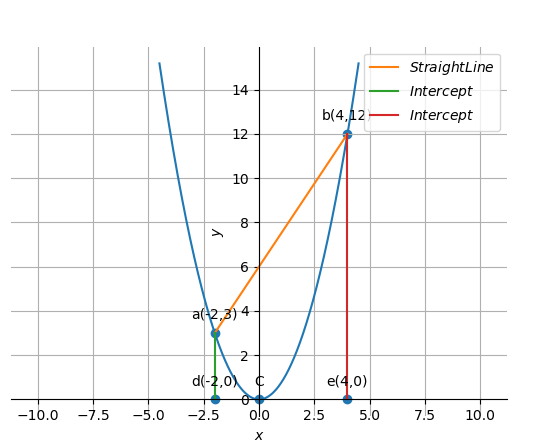
\includegraphics[width=\columnwidth]{chapters/12/8/3/7/figs/conic.png}
		\caption{}
		\label{fig:12/8/3/7}
  	\end{figure}
\iffalse
\vspace{5mm}
%-----------------------------solution---------------------------
\raggedright \textbf{SOLUTION}:\vspace{2mm}\\

%---------given----------------%
\raggedright \textbf{Given}:\vspace{2mm}\\
Equation of parabola is \\\vspace{1mm}
\begin{align}
4y=3x^2
\end{align}
Equation of line is \\ \vspace{1mm}
\begin{align}
2y=3x+12
\end{align}
%-------------To find ------------------%
\textbf{To Find }\vspace{2mm}\\
To find the intersection points and area enclosed by the parabola and line shown in figure\vspace{2mm}  \\ 
%--------------steps----------------------%
\textbf{STEP-1}\vspace{2mm}\\
The given parabola can be expressed as conics with parameters,\\ \vspace{1mm}
\begin{align}
	\vec{x}^{\top}\vec{V}\vec{x} + 2\vec{u}^{\top} \vec{x} + f = 0
\end{align}
\fi
The parameters of the given conic are
\begin{align}
\vec{V}=\myvec{
3 & 0\\
0 & 0
},
\vec{u}=\myvec{0\\-2},
f=0.
\end{align} 
For the line, the parameters are
\iffalse
\textbf{STEP-2}\vspace{2mm}\\
the given line equation can be written as\\ 
\begin{align} 
	\vec{n}^{\top}\vec{X}=c
\end{align}
Where
\begin{align}
\vec{n}=\myvec{-3\\2},\vec{m}=\myvec{2\\3}
\end{align}
\textbf{STEP-3}\vspace{2mm}\\
The points of intersection of the line, \\ 
\begin{align}
L: \quad \vec{x} = \vec{q} + \kappa \vec{m} \quad \kappa \in \mathbb{R}
\end{align}
with the conic section, \\ 
\begin{align}
	\vec{x}^{\top}\vec{V}\vec{x} + 2\vec{u}^{\top} \vec{x} + f = 0
\end{align}
are given by \\
\begin{align}
\vec{x}_i = \vec{q} + \kappa_i \vec{m}
\end{align}
where, \\
{\tiny
\begin{multline}
\kappa_i = \frac{1}
{
\vec{m}^T\vec{V}\vec{m}
}
\lbrak{-\vec{m}^T\brak{\vec{V}\vec{q}+\vec{u}}}
\\
\pm
\rbrak{\sqrt{
\sbrak{
\vec{m}^T\brak{\vec{V}\vec{q}+\vec{u}}
}^2
-
\brak
{
\vec{q}^T\vec{V}\vec{q} + 2\vec{u}^T\vec{q} +f
}
\brak{\vec{m}^T\vec{V}\vec{m}}
}
}
\end{multline}
}
On substituting\\
\fi
\begin{align}
\vec{h} = \myvec{
-2\\
3
},
\vec{m} = \myvec{2 \\ 3}
\end{align}
\iffalse
With the given parabola as in eq(3),(4),(5),\\ 

The value of $\kappa$ ,\\
\fi
yielding
\begin{align}
    \mu=-2.5,2.7
\end{align}
upon substitution in \eqref{eq:tangent_roots}
resulting in the points of intersection
\iffalse
by substituting eq(13) in eq(6)we get the
points of intersection of line with parabola \\
\fi
\begin{align}
    \vec{A}=\myvec{
-2\\
3
    },
    \vec{B}=\myvec{
4\\
12
    }.
\end{align}
From Fig. 
		\ref{fig:12/8/3/7},
		\iffalse
\textbf{Result}
\begin{center}
 \includegraphics[scale=0.5]{conic.png}    
 \end{center}\vspace{1mm}
 From the figure,\\ \vspace{1mm}
Total area of portion is given by, \\ \vspace{1mm}
Total Area=(area enclosed by the line)-(area of parabola under the line )

\subsection*{Area Under the line}
\fi
the desired area is 
\begin{align}
\int_{-2}^{4} \frac{3x+12}{2} \,dx
-\int_{-2}^{4}\frac{3x^2}{4} \,dx 
= 27 
\end{align}
\iffalse
 \vspace{2mm} \textbf{Construction}
\begin{center}
\setlength{\arrayrulewidth}{0.5mm}
\setlength{\tabcolsep}{6pt}
\renewcommand{\arraystretch}{1.5}
    \begin{tabular}{|l|c|}
    \hline 
    \textbf{Points} & \textbf{coordinates} \\ \hline
   B & $\myvec{
   4\\
   12
   } $ \\\hline
   A & $\myvec{
   -2\\
   3
   } $ \\\hline
      \end{tabular}
  \end{center}
  \end{multicols}
 
Get the python code of the figures from

\begin{table}[h]
\large
\centering
\framebox{
\url{https://github.com/chandana531/cchandana_fwc/blob/main/conic_assignment/code/conic.py}}
\bibliographystyle{ieeetr}
\end{table} 
 
\end{document}
 
\fi

\item 
\label{chapters/12/8/3/8}
\iffalse
\documentclass[10pt,a4paper]{report}
%\usepackage[latin1]{inputenc}
\usepackage[utf8]{inputenc}
\usepackage{amsmath}
\usepackage{amsfonts}
\usepackage{amssymb}
\usepackage{graphicx}
\usepackage{multicol}
\usepackage{tabularx}
\usepackage{tikz}
\usetikzlibrary{arrows,shapes,automata,petri,positioning,calc}
\usepackage{hyperref}
\usepackage{tikz}
\usetikzlibrary{matrix,calc}
\usepackage[margin=0.5in]{geometry}
% ---- power functions -----% 
\newcommand{\myvec}[1]{\ensuremath{\begin{pmatrix}#1\end{pmatrix}}}
\let\vec\mathbf

\providecommand{\norm}[1]{\left\lVert#1\right\rVert}
\providecommand{\abs}[1]{\left\vert#1\right\vert}
\let\vec\mathbf

\newcommand{\mydet}[1]{\ensuremath{\begin{vmatrix}#1\end{vmatrix}}}
\providecommand{\brak}[1]{\ensuremath{\left(#1\right)}}
\providecommand{\lbrak}[1]{\ensuremath{\left(#1\right.}}
\providecommand{\rbrak}[1]{\ensuremath{\left.#1\right)}}
\providecommand{\sbrak}[1]{\ensuremath{{}\left[#1\right]}}
%-------end power functions----%
\newenvironment{Figure}
  {\par\medskip\noindent\minipage{\linewidth}}
  {\endminipage\par\medskip}
\begin{document}
%--------------------logo figure-------------------------%
\begin{figure*}[!tbp]
  \centering
  \begin{minipage}[b]{0.4\textwidth}
    
\includegraphics[scale=0.05]{iitlogo.jpg} 
  \end{minipage}
  \hfill
  \vspace{5mm}\begin{minipage}[b]{0.4\textwidth}
\raggedleft  
\includegraphics[scale=0.05]{nrc.png}  \

  \end{minipage}\vspace{0.2cm}
\end{figure*}
%--------------------name & rollno-----------------------
\raggedright \textbf{Name}:\hspace{1mm} D. Siva Krishna\hspace{3cm} \Large \textbf{Assignment-6}\hspace{2.5cm} % 
\normalsize \textbf{Roll No.} :\hspace{1mm} FWC22065\vspace{1cm}
\begin{multicols}{2}

%----------------problem statement--------------%
\raggedright \textbf{Problem Statement:}\vspace{2mm}
\raggedright \\
\fi
	Find the area of the smaller region bounded by the ellipse $\frac{x^2}{9}+\frac{y^2}{4}=1$
and the line $\frac{x}{3}+\frac{y}{2}=1$.\\
\solution
	\begin{figure}[!h]
		\centering
 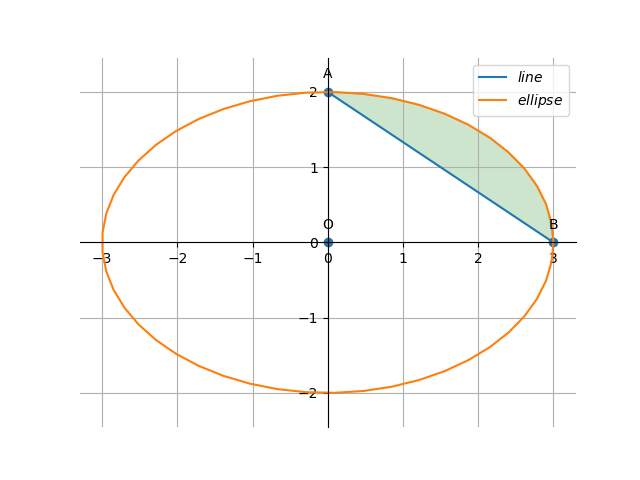
\includegraphics[width=\columnwidth]{chapters/12/8/3/8/figs/conic_fig.png}
		\caption{}
		\label{fig:12/8/3/8}
  	\end{figure}
\iffalse
\vspace{5mm}
%-----------------------------solution---------------------------
\raggedright \textbf{SOLUTION}:\vspace{2mm}\\
\section{Without numericals}
%---------given----------------%
\raggedright \textbf{Given}:\vspace{2mm}\\
The general equation of ellipse is \\\vspace{1mm}
\begin{align}
\frac{x^2}{a^2}+\frac{y^2}{b^2}=1
\end{align}
The general equation of line is \\ \vspace{1mm}
\begin{align}
\frac{x}{a}+\frac{y}{b}=1
\end{align}
%-------------To find ------------------%
\textbf{To Find }\vspace{2mm}\\
To find the intersection points and area of shaded region shown in figure\vspace{2mm}  \\ 
%--------------steps----------------------%
\textbf{STEP-1}\vspace{2mm}\\
\fi
The given ellipse can be expressed as conics with parameters
\begin{align}
\vec{V}=\myvec{
b^2 & 0\\
0 & a^2
},
\vec{u}=0,
f=-(a^2b^2).
\end{align} 
The line parameters are
\iffalse
\begin{align} 
	\vec{x}=\begin{pmatrix}a \\ 0 \\ \end{pmatrix}+k\begin{pmatrix}\frac{1}{b} \\ -\frac{1}{a} \\ \end{pmatrix}
\end{align}

\textbf{STEP-3}\vspace{2mm}\\
The points of intersection of the line, \\ 
\begin{align}
L: \quad \vec{x} = \vec{q} + \kappa \vec{m} \quad \kappa \in \mathbb{R}
\end{align}
with the conic section, \\ 
\begin{align}
	\vec{x}^{\top}\vec{V}\vec{x} + 2\vec{u}^{\top} \vec{x} + f = 0
\end{align}
are given by \\
\begin{align}
\vec{x}_i = \vec{q} + \kappa_i \vec{m}
\end{align}
where, \\
{\tiny
\begin{multline}
\kappa_i = \frac{1}
{
\vec{m}^T\vec{V}\vec{m}
}
\lbrak{-\vec{m}^T\brak{\vec{V}\vec{q}+\vec{u}}}
\\
\pm
\rbrak{\sqrt{
\sbrak{
\vec{m}^T\brak{\vec{V}\vec{q}+\vec{u}}
}^2
-
\brak
{
\vec{q}^T\vec{V}\vec{q} + 2\vec{u}^T\vec{q} +f
}
\brak{\vec{m}^T\vec{V}\vec{m}}
}
}
\end{multline}
}
On substituting\\
\fi
\begin{align}
\vec{h} &= \myvec{
a\\
0
},
\vec{m} = \myvec{\frac{1}{b} \\ -\frac{1}{a}}.
\end{align}
\iffalse
With the given ellipse as in eq(3),(4),(5),\\ 

The value of $\kappa$ ,\\
\fi
Substituting the given parameters in \eqref{eq:tangent_roots},
\begin{align}
    \mu=0,-6
\end{align}
yielding the points of intersection
\iffalse
by substituting eq(13) in eq(6)we get the
points of intersection of line with ellipse \\
\fi
\begin{align}
    \vec{A}=\myvec{
a\\
0
    },
    \vec{B}=\myvec{
0\\
b
    }.
\end{align}
From Fig. 
		\ref{fig:12/8/3/8},
		\iffalse
\section{Substituting the numericals according to the problem}
\begin{align}
a=3, \vspace{2mm}
b=2\\
\vec{\textbf{V}}=\myvec{4\hspace{2mm}0\\ 0 \hspace{2mm} 9}, \vspace{2mm}
\vec{\textbf{u}}=0, \vspace{2mm}
f = -36\\
\vec{\textbf{q}}=\myvec{3\\0}, \vspace{2mm}
\vec{\textbf{m}}=\myvec{\frac{1}{2}\\-\frac{1}{3}}, \vspace{2mm}\\
\vec{\textbf{A}}=\myvec{0\\2}, \vspace{2mm}
\vec{\textbf{B}}=\myvec{3\\o}
\end{align}
\textbf{Result}
\begin{center}
 \includegraphics[scale=0.5]{conic_fig.png}    
 \end{center}\vspace{1mm}
 From the figure,\\ \vspace{1mm}
Total area of portion is given by, \\ \vspace{1mm}
Total Area=(area of ellipse in first quadrant)-(area of a triangle\textbf{AOB})

\subsection*{Area of ellipse}
\fi
the desired
area is
\begin{align} 
%A2=\int_{0}^{a}\frac{b}{a}\sqrt{a^2-x^2} \,dx 
%\\
\int_{0}^{3}\frac{2}{3}\sqrt{9-x^2} \,dx 
%\implies A1=\int_{0}^{a} \frac{b}{a}(a-x) \,dx\\
-\int_{0}^{3} \frac{2}{3}(3-x) \,dx
	= 3\brak{\frac{\pi}{2}-1}
\end{align}
\iffalse
 \vspace{2mm} \textbf{Construction}
\begin{center}
\setlength{\arrayrulewidth}{0.5mm}
\setlength{\tabcolsep}{6pt}
\renewcommand{\arraystretch}{1.5}
    \begin{tabular}{|l|c|}
    \hline 
    \textbf{Points} & \textbf{coordinates} \\ \hline
   B & $\myvec{
   a\\
   0
   } $ \\\hline
   A & $\myvec{
   0\\
   b
   } $ \\\hline
      \end{tabular}
  \end{center}
  \end{multicols}
 
\textbf{Download code}

\begin{table}[h]
\large
\centering
\framebox{
\url{https://github.com/Siva Krishna/blob/main/conics/code/conic.py}}
\bibliographystyle{ieeetr}
\end{table} 
 
\end{document}
\fi

\item 
\label{chapters/12/8/3/9}
\documentclass[10pt,a4paper]{report}
%\usepackage[latin1]{inputenc}
\usepackage[utf8]{inputenc}
\usepackage{amsmath}
\usepackage{amsfonts}
\usepackage{amssymb}
\usepackage{graphicx}
\usepackage{multicol}
\usepackage{tabularx}
\usepackage{tikz}
\usetikzlibrary{arrows,shapes,automata,petri,positioning,calc}
\usepackage{hyperref}
\usepackage{tikz}
\usetikzlibrary{matrix,calc}
\usepackage[margin=0.5in]{geometry}
% ---- power functions -----% 
\newcommand{\myvec}[1]{\ensuremath{\begin{pmatrix}#1\end{pmatrix}}}
\let\vec\mathbf

\providecommand{\norm}[1]{\left\lVert#1\right\rVert}
\providecommand{\abs}[1]{\left\vert#1\right\vert}
\let\vec\mathbf

\newcommand{\mydet}[1]{\ensuremath{\begin{vmatrix}#1\end{vmatrix}}}
\providecommand{\brak}[1]{\ensuremath{\left(#1\right)}}
\providecommand{\lbrak}[1]{\ensuremath{\left(#1\right.}}
\providecommand{\rbrak}[1]{\ensuremath{\left.#1\right)}}
\providecommand{\sbrak}[1]{\ensuremath{{}\left[#1\right]}}
%-------end power functions----%
\newenvironment{Figure}
  {\par\medskip\noindent\minipage{\linewidth}}
  {\endminipage\par\medskip}
\begin{document}
%--------------------logo figure-------------------------%
\begin{figure*}[!tbp]
  \centering
  \begin{minipage}[b]{0.4\textwidth}
    
\includegraphics[scale=0.05]{fig/iitlogo.jpg} 
  \end{minipage}
  \hfill
  \vspace{5mm}\begin{minipage}[b]{0.4\textwidth}
\raggedleft  
\includegraphics[scale=0.05]{fig/nrc.png}  \

  \end{minipage}\vspace{0.2cm}
\end{figure*}
%--------------------name & rollno-----------------------
\raggedright \textbf{Name}:\hspace{1mm} kanekal kousar\hspace{3cm} \Large \textbf{Conic Assignment}\hspace{2.5cm} % 
\normalsize \textbf{Roll No.} :\hspace{1mm} FWC22063\vspace{1cm}
\begin{multicols}{2}

%----------------problem statement--------------%
\raggedright \textbf{Problem Statement:}\vspace{2mm}
\raggedright \\Find the area of the smaller region bounded by the ellipse $\frac{x^2}{a^2}+\frac{y^2}{b^2}=1$
and the line $\frac{x}{a}+\frac{y}{b}=1$\\
\vspace{5mm}
%-----------------------------solution---------------------------
\raggedright \textbf{SOLUTION}:\vspace{2mm}\\

%---------given----------------%
\raggedright \textbf{Given}:\vspace{2mm}\\
Equation of ellipse is \\\vspace{1mm}
\begin{align}
\frac{x^2}{a^2}+\frac{y^2}{b^2}=1
\end{align}
Equation of line is \\ \vspace{1mm}
\begin{align}
\frac{x}{a}+\frac{y}{b}=1
\end{align}
%-------------To find ------------------%
\textbf{To Find }\vspace{2mm}\\
To find the intersection points and area of shaded region shown in figure\vspace{2mm}  \\ 
%--------------steps----------------------%
\textbf{STEP-1}\vspace{2mm}\\
The given ellipse can be expressed as conics with parameters,\\ \vspace{1mm}
\begin{align}
\vec{V}=\myvec{
b^2 & 0\\
0 & a^2
}
\end{align}

\begin{align}
\vec{u}=0
\end{align} 
\begin{align}
f=-(a^2b^2)
\end{align} \vspace{2mm}


\textbf{STEP-2}\vspace{2mm}\\
the given line equation can be written as\\ 
\begin{align} 
	\vec{x}=\begin{pmatrix}a \\ 0 \\ \end{pmatrix}+k\begin{pmatrix}\frac{1}{b} \\ -\frac{1}{a} \\ \end{pmatrix}
\end{align}

\textbf{STEP-3}\vspace{2mm}\\
The points of intersection of the line, \\ 
\begin{align}
L: \quad \vec{x} = \vec{q} + \kappa \vec{m} \quad \kappa \in \mathbb{R}
\end{align}
with the conic section, \\ 
\begin{align}
	\vec{x}^{\top}\vec{V}\vec{x} + 2\vec{u}^{\top} \vec{x} + f = 0
\end{align}
are given by \\
\begin{align}
\vec{x}_i = \vec{q} + \kappa_i \vec{m}
\end{align}
where, \\
{\tiny
\begin{multline}
\kappa_i = \frac{1}
{
\vec{m}^T\vec{V}\vec{m}
}
\lbrak{-\vec{m}^T\brak{\vec{V}\vec{q}+\vec{u}}}
\\
\pm
\rbrak{\sqrt{
\sbrak{
\vec{m}^T\brak{\vec{V}\vec{q}+\vec{u}}
}^2
-
\brak
{
\vec{q}^T\vec{V}\vec{q} + 2\vec{u}^T\vec{q} +f
}
\brak{\vec{m}^T\vec{V}\vec{m}}
}
}
\end{multline}
}
On substituting\\
\begin{align}
\vec{q} &= \myvec{
a\\
0
} 
\end{align}
\begin{align}
\vec{m} = \myvec{\frac{1}{b} \\ -\frac{1}{a}}
\end{align}
With the given ellipse as in eq(3),(4),(5),\\ 

The value of $\kappa$ ,\\
\begin{align}
    \kappa =0,-6
\end{align}
by substituting eq(13) in eq(6)we get the
points of intersection of line with ellipse \\
\begin{align}
    \vec{A}=\myvec{
a\\
0
    }
\end{align}
\begin{align}
    \vec{B}=\myvec{
0\\
b
    }
\end{align}
\textbf{Result}
\begin{center}
 \includegraphics[scale=0.5]{fig/conic_fig.png}    
 \end{center}\vspace{1mm}
 From the figure,\\ \vspace{1mm}
Total area of portion is given by, \\ \vspace{1mm}
Total Area=(area of ellipse in first quadrant)-(area of a triangle\textbf{AOB})

\subsection*{Area of triangle}

\begin{align}
\implies A1=\int_{0}^{a} \frac{b}{a}(a-x) \,dx
\end{align}
by solving the above equation we get area of triangle \textbf{$\frac{ab}{2}$}
\subsection*{Area of ellipse}

\begin{align} 
\implies A2=\int_{0}^{a}\frac{b}{a}\sqrt{a^2-x^2} \,dx 
\end{align}
by solving the above equation we get area of ellipse $\frac{\pi ab}{4}$

the total area is

\vspace{3mm}
$\implies A=\frac{\pi ab}{4}-\frac{ab}{2}$\vspace{3mm}

The area of the smaller region is ,
\begin{align}
\hspace{-4.25cm}A= \frac{ab}{2}(\frac{\pi}{2}-1)
\end{align}
 \vspace{2mm} \textbf{Construction}
\begin{center}
\setlength{\arrayrulewidth}{0.5mm}
\setlength{\tabcolsep}{6pt}
\renewcommand{\arraystretch}{1.5}
    \begin{tabular}{|l|c|}
    \hline 
    \textbf{Points} & \textbf{coordinates} \\ \hline
   B & $\myvec{
   a\\
   0
   } $ \\\hline
   A & $\myvec{
   0\\
   b
   } $ \\\hline
      \end{tabular}
  \end{center}
  \end{multicols}
 
Get the python code of the figures from

\begin{table}[h]
\large
\centering
\framebox{
\url{https://github.com/kkousar/KOUSAR_FWC/blob/main/conics/code/conic.py}}
\bibliographystyle{ieeetr}
\end{table} 
 
\end{document}
 
\item 
\label{chapters/12/8/3/10}
\iffalse
\documentclass[journal,10pt,twocolumn]{article}
\usepackage{graphicx}
\usepackage[margin=0.5in]{geometry}
\usepackage[cmex10]{amsmath}
\usepackage{array}
\usepackage{booktabs}
\usepackage{mathtools}
\title{\textbf{Conic section Assignment}}
\author{P.Revathi}
\date{October 2022}


\providecommand{\norm}[1]{\left\lVert#1\right\rVert}
\providecommand{\abs}[1]{\left\vert#1\right\vert}
\let\vec\mathbf
\newcommand{\myvec}[1]{\ensuremath{\begin{pmatrix}#1\end{pmatrix}}}
\newcommand{\mydet}[1]{\ensuremath{\begin{vmatrix}#1\end{vmatrix}}}
\providecommand{\brak}[1]{\ensuremath{\left(#1\right)}}
\providecommand{\lbrak}[1]{\ensuremath{\left(#1\right.}}
\providecommand{\rbrak}[1]{\ensuremath{\left.#1\right)}}
\providecommand{\sbrak}[1]{\ensuremath{{}\left[#1\right]}}

\begin{document}

\maketitle
\paragraph{\textit{Problem Statement} -
\fi
Find the area of the region bounded by the curve $x^2=y$ and the lines $y=x+2$ and the $x$ axis.
\\
\solution 
	\begin{figure}[!h]
		\centering
 \includegraphics[width=\columnwidth]{chapters/12/8/3/10/figs/conics1.png}
		\caption{}
		\label{fig:12/8/3/10}
  	\end{figure}
\iffalse

\section*{\large Solution}

\begin{figure}[h]
\centering
\includegraphics[width=1\columnwidth]{conics1.png}

%\caption{The parabola formed by the curve $y^2 = 9x$ and the lines x=2 and x=4}
\label{fig:parabola}
\end{figure}

The given equation of parabola $x^2 = y$ can be written in the general quadratic form as
\begin{align}
    \label{eq:conic_quad_form}
    \vec{x}^{\top}\vec{V}\vec{x}+2\vec{u}^{\top}\vec{x}+f=0
    \end{align}
where
The parameters of the given conic are
\begin{align}
 \vec{V} = \myvec{1 & 0\\0 & 0},
 \vec{u} = \myvec{0\\-0.5},
 f = 0
\end{align}
The points of intersection of the line 
\begin{align}
 L: \quad \vec{x} = \vec{q} + \mu \vec{m} \quad \mu \in \mathbf{R}
\label{eq:conic_tangent}
\end{align}
with the conic section are given by
\begin{align}
\vec{x}_i = \vec{q} + \mu_i \vec{m}
\label{eq:conic_tangent_pts}
\end{align}
%
where
{\tiny
\begin{multline}
\mu_i = \frac{1}
{
\vec{m}^T\vec{V}\vec{m}
}
\lbrak{-\vec{m}^T\brak{\vec{V}\vec{q}+\vec{u}}}
\\
\pm
\rbrak{\sqrt{
\sbrak{
\vec{m}^T\brak{\vec{V}\vec{q}+\vec{u}}
}^2
-
\brak
{
\vec{q}^T\vec{V}\vec{q} + 2\vec{u}^T\vec{q} +f
}
\brak{\vec{m}^T\vec{V}\vec{m}}
}
}
\label{eq:tangent_roots}
\end{multline}
}
The parameters of the line $y=x+2$ are
\begin{align}
\vec{h}=\myvec{0\\2},
\vec{m}=\myvec{1\\1}
\end{align}
yielding
\begin{align}
\mu_i=-2
\end{align}
upon substituting in \eqref{eq:tangent_roots}.     The points of intersection of this line with the conic are
\begin{align}
\vec{a_0}=\myvec{2\\4},
\vec{a_1}=\myvec{-1\\1}
\end{align}
Similarly, 
Given line equation y=x+2\\

$$x-y=-2$$\\
$$\vec{n}^{t}\vec{x}=c$$\\
$$\vec{x}=\vec{A}+\lambda \vec{m}$$\\
%\end{centre}


$$\vec{x}=\begin{pmatrix}
-2\\ 
0
\end{pmatrix}+\mu \begin{pmatrix}
1\\ 
1
\end{pmatrix}$$\\

Substitute the x value in the quadratic equation then we get a quadratic equations
\begin{align}
    \label{eq:conic_quad_form}
    \vec{x}^{\top}\vec{V}\vec{x}+2\vec{u}^{\top}\vec{x}+f=0
    \end{align}
    
$$\mu ^{2}-3\mu +2=0\\$$
$$\mu =1,2\\$$
$$\mu ^{2}-\mu\\$$
$$\mu =1,0\\$$
The resultant x values are\\
$$\vec{x}=\begin{pmatrix}
-2\\ 
0
\end{pmatrix}$$\\
$$\vec{x}=\begin{pmatrix}
-1\\ 
1
\end{pmatrix}$$\\
$$\vec{x}=\begin{pmatrix}
0\\ 
2
\end{pmatrix}$$

Area of the parabola in between the lines parabola and y=x+2 is given by
\begin{align}
\implies A_1=\int_{-2}^{-1} \ x+2 \,dx
\end{align}

\begin{align}
\implies A_2=\int_{-1}^{0} \ x^2 \,dx
\end{align}
\begin{align}
\implies A_1+A_1=\int_{-2}^{-1} \ x+2 \,dx+\int_{-1}^{0} \ x^2 \,dx
\end{align}
\begin{align}
\implies A_1+ A_2=\frac{5}{6}sq units
\end{align}

\end{document}
\fi

\item 
\label{chapters/12/8/3/17}
\iffalse
\def\mytitle{MATRICES USING PYTHON(CONIC)}
\def\myauthor{R.Radhika}
\def\contact{r170234@rguktrkv.ac.in}
\def\mymodule{Future Wireless Communication (FWC)}
\documentclass[10pt, a4paper]{article}
\usepackage[a4paper,outer=1.5cm,inner=1.5cm,top=1.75cm,bottom=1.5cm]{geometry}
\twocolumn
\usepackage{graphicx}
\graphicspath{{./images/}}
\usepackage[colorlinks,linkcolor={black},citecolor={blue!80!black},urlcolor={blue!80!black}]{hyperref}
\usepackage[parfill]{parskip}
\usepackage{lmodern}
\usepackage{tikz}
	\usepackage{physics}
%\documentclass[tikz, border=2mm]{standalone}
%\usepackage{karnaugh-map}
%\documentclass{article}
\usepackage{tabularx}
%\usepackage{circuitikz}
\usepackage{enumitem}
\usetikzlibrary{calc}
\usepackage{amsmath}
\usepackage{amssymb}
\renewcommand*\familydefault{\sfdefault}
\usepackage{watermark}
\usepackage{lipsum}
\usepackage{xcolor}
\usepackage{listings}
\usepackage{float}
\usepackage{titlesec}
\providecommand{\mtx}[1]{\mathbf{#1}}
\titlespacing{\subsection}{1pt}{\parskip}{3pt}
\titlespacing{\subsubsection}{0pt}{\parskip}{-\parskip}
\titlespacing{\paragraph}{0pt}{\parskip}{\parskip}
\newcommand{\figuremacro}[5]{
    \begin{figure}[#1]
        \centering
        \includegraphics[width=#5\columnwidth]{#2}
        \caption[#3]{\textbf{#3}#4}
        \label{fig:#2}
    \end{figure}
}

\newcommand{\myvec}[1]{\ensuremath{\begin{pmatrix}#1\end{pmatrix}}}
\let\vec\mathbf
\lstset{
frame=single, 
breaklines=true,
columns=fullflexible
}

\title{\mytitle}
\author{\myauthor\hspace{1em}\\\contact\\FWC22066\hspace{6.5em}IITH\hspace{0.5em}\mymodule\hspace{6em}Assignment}
\begin{document}
	\maketitle
	\tableofcontents
   \section{Problem}
   \fi
Find   the area bounded by the curve $y=x|x|, x$-axis and the ordinates $x$=-1 and $x$=1.
\\
\solution 
	\begin{figure}[!h]
		\centering
 \includegraphics[width=\columnwidth]{chapters/12/8/3/17/figs/conicfig.pdf}
		\caption{}
		\label{fig:12/8/3/17}
  	\end{figure}
   \iffalse
[Hint: y=$x^2$ if $x>0$  and y=$-x^2$ if $x<0$]
   					
\section{Construction}
  \includegraphics[scale=0.47]{conicfig.pdf}
  	\begin{center}
  Figure of construction
  	\end{center}
  \section{Solution}
  
\raggedright\large{ Draw the ordinates by using $x$=1 and $x$=-1. Then we need to draw  two parabolas using  given hint [Hint: y=$x^2$ if $x>0$  and y=$-x^2$ if $x<0$]for that we need to find out the area bounded by the curve  y=$x|x|$  .}
\vspace{2mm}\\
\raggedright\large{Then the limits from -1 to 1  and the points(-1,-1),(1,1)}\vspace{2mm}\\
The standard conic equation\\
\begin{align}
\vec{x}^{\top}\vec{V}\vec{x}+2\vec{u}^{\top}\vec{x}+f=0
\end{align}
\begin{align}
\vec{x}^{\top}\vec{V}\vec{x}+2\vec{u_1}^{\top}\vec{x}+f_1=0
\end{align}
\fi
The parameters of the given conics are
\begin{align}
	\vec{V}_1&=\myvec{1&0\\0&0} ,\vec{u_1}=\myvec{0\\-\frac{1}{2}},  f_1=0
	\\
	\vec{V}_2&=\myvec{-1&0\\0&0} ,\vec{u_2}=\myvec{0\\-\frac{1}{2}},  f_2=0
\end{align}
The determinant equation for the intersection of two conics is 
\iffalse
\begin{align}
|\myvec{\vec{V_1}+\mu{\vec{V_2}}&\vec{u_1}+\mu{\vec{u_2}}\\\vec{u_1}+\mu{\vec{u_2}}&0}|
\end{align}
substitute eq 3 and 4 in eq 6\\
\fi
\begin{align}
\mydet{1-\mu&0&0\\0&0&-\frac{1}{2}-\frac{\mu}{2}\\0&-\frac{1}{2}-\frac{\mu}{2}&0} = 0
\end{align}
yielding,
\begin{align}
	\mu^3+\mu^2-\mu-1&=0
	\\
	\implies
	\mu&=-1, 1, 1
\end{align}
\iffalse
\begin{align}
|\vec{V_1}+\mu\vec{V_2}|<0
\end{align}
substitute $\vec{V_1}$ and $\vec{V_2}$ in eq-9\\
we get 0\\
\begin{align}
\vec{x}=\vec{q}+\mu{\vec{m}}
\end{align}
\begin{align}
q=\vec{V^{-1}}(k\vec{n}-\vec{u})
\end{align}
\begin{align}
k=\pm\sqrt{\frac{\norm{\vec{u_2}}^2\vec{V}-f}{\vec{n}^{\top}\vec{V^{-1}}\vec{n}}}
\end{align}
$\vec{n}=\myvec{1\\-1}$\\
$\vec{m}=\myvec{1\\1}$\\

by solving eq 10 and 11 we get\\
\begin{align}
\vec{q}=\myvec{0\\0}
\end{align}


 Given equation :  y=$x|x|$\\

We know that \\
\begin{equation}
   |x| =
    \begin{cases}
      x, & {x\geq0}\\
      -x & {x<0}\\
    \end{cases}       
\end{equation}

	Therefore,
\begin{equation}
   y=x|x| =
    \begin{cases}
      xx, & {x\geq0}\\
      x(-x) & {x<0}\\
    \end{cases}       
\end{equation}
\begin{equation}
   y =
    \begin{cases}
      x^2, & {x\geq0}\\
      -x^2 & {x<0}\\
    \end{cases}       
\end{equation}
Area Required=Area ABO+Area DCO\\
\textbf{Area of DCO}

Area  : \[ \int_{-1}^{1} y \,dx \]

Here, y=$x|x|$

Therefore Area DCO: \[ \int_{-1}^{0} -x^2 \,dx \]

 yielding ,\\
 
   -1/3 \\
 
 $|(-1/3)|$=1/3\\
 
 Area of DCO= 1/3

\textbf{Area  of ABO}: \[ \int_{0}^{1} x^2 \,dx \]

    yielding 1/3\\
   
     
     Area of ABO= 1/3
     

\textbf{Required Area=ABO+DCO}:
  1/3+1/3=2/3
Below python code realizes the above construction 

\begin{table}[h!]
    \begin{tabular}{|c|}
    \hline
         https://github.com/Radhikarkv/fwcproject.git\\
	\hline
    \end{tabular}
\end{table}
\end{document}
\fi

\item 
\label{chapters/12/8/3/18}
\iffalse
\documentclass[10pt,a4paper]{report}
%\usepackage[latin1]{inputenc}
\usepackage[utf8]{inputenc}
\usepackage{amsmath}
\usepackage{amsfonts}
\usepackage{amssymb}
\usepackage{graphicx}
\usepackage{multicol}
\usepackage{tabularx}
\usepackage{tikz}
\usetikzlibrary{arrows,shapes,automata,petri,positioning,calc}
\usepackage{hyperref}
\usepackage{tikz}
\usetikzlibrary{matrix,calc}
\usepackage[margin=0.5in]{geometry}
% ---- power functions -----% 
\newcommand{\myvec}[1]{\ensuremath{\begin{pmatrix}#1\end{pmatrix}}}
\let\vec\mathbf
%\providecommand $${\norm}[1]{\left\lVert#1\right\rVert}$$
\providecommand{\abs}[1]{\left\vert#1\right\vert}
\let\vec\mathbf

\newcommand{\mydet}[1]{\ensuremath{\begin{vmatrix}#1\end{vmatrix}}}
\providecommand{\brak}[1]{\ensuremath{\left(#1\right)}}
\providecommand{\lbrak}[1]{\ensuremath{\left(#1\right.}}
\providecommand{\rbrak}[1]{\ensuremath{\left.#1\right)}}
\providecommand{\sbrak}[1]{\ensuremath{{}\left[#1\right]}}
%-------end power functions----%
\newenvironment{Figure}
  {\par\medskip\noindent\minipage{\linewidth}}
  {\endminipage\par\medskip}
\begin{document}
%--------------------name & rollno-----------------------
\raggedright \textbf{Name}:\hspace{1mm} A.SUSI\hspace{3cm} \Large \textbf{Matrices Using Python}\hspace{2.5cm} % 
\normalsize \textbf{Roll No.} :\hspace{1mm} FWC22067\vspace{1cm}
\begin{multicols}{2}

%----------------problem statement--------------%

\raggedright \textbf{Problem Statement:}\vspace{2mm}
\raggedright \\
\fi
	Find the area of the circle $x^2 + y^2 = 16$ exterior to the parabola $y^2 = 6x$.\\
	\solution
	\begin{figure}[!h]
		\centering
 \includegraphics[width=\columnwidth]{chapters/12/8/3/18/figs/cp.jpg}
		\caption{}
		\label{fig:12/8/3/18}
  	\end{figure}
	\iffalse
\vspace{5mm}
%-----------------------------solution---------------------------
\raggedright \textbf{SOLUTION}:\vspace{2mm}\\

%---------given----------------%
\raggedright \textbf{Given}:\vspace{2mm}\\
Equation of circle is \\\vspace{1mm}
\begin{align}
x^2 + y^2 = 16
\end{align}
Equation of Parabola is \\ \vspace{1mm}
\begin{align}
y^2 = 6x 
\end{align}
From (2) we can say that Parabola is concave towards positive xaxis.\\ \vspace{2mm}
From equation (1) radius of circle is,\\ \vspace{1mm}
\begin{align}
r= 4
\end{align}

%-------------To find ------------------%
\textbf{To Find }\vspace{2mm}\\
To find the intersection points and area of unshaded region shown in figure\vspace{2mm}  \\ 
%--------------steps----------------------%
\textbf{STEP-1}\vspace{2mm}\\
\fi
The given circle and parabola can be expressed as conics with respectiveparameters
\begin{align}
	\vec{V}_1&=\vec{I},
\vec{u_1}=0,
f_1=-16,
\\
	\vec{V}_2&=\myvec{
0 & 0\\
0 & 1
},
\vec{u_2}= -\myvec{
3\\
0
},
f_2=0
\end{align} 
The determinant of the intersection of the given conics is 
\iffalse
\begin{align}
	\vec{x}^{\top}\brak{\vec{V}_1 + \mu\vec{V}_2}\vec{x}+2 \brak{\vec{u}_1+\mu \vec{u}_2}^{\top} \vec{x} 
	\\
	+ \brak{f_1+\mu f_2}= 0
    \end{align}
    
\begin{align}
\vec{V}_1+\mu\vec{V}_2= \myvec{
1 & 0\\
0 & \mu+1
}
\end{align}
\begin{align}
\vec{u}_1+\mu\vec{u}_2= -\myvec{
3\mu\\
0
}
\end{align}
\begin{align}
f_1+\mu f_2= -16
\end{align}
This conic is a single straight line if and only if, \\ \vspace{1mm}
\begin{align}
\mydet{\vec{V}_1 + \mu\vec{V}_2 & \vec{u}_1+\mu \vec{u}_2\\ \brak{\vec{u}_1+\mu \vec{u}_2}^{\top} & f_1 + \mu f_2} &= 0
\end{align}
And,\\
\begin{align}
\mydet{\vec{V}_1 + \mu\vec{V}_2} &= 0
\end{align}
Substituting equation (13),(14) and (15) in equation (16)\\ \vspace{1mm}
We get,\\ \vspace{1mm}
\fi
\begin{align}
\implies \mydet{1& 0 & -3\mu\\ 
0 & 1+\mu & 0 \\
-3\mu & 0 & -16
} &= 0
\end{align}
yielding
\begin{align}
	9\mu^3 + 9\mu^2 + 16\mu + 16&=0
	\\
	\text{or, }
    \mu = -1
\end{align}
\iffalse
 Thus, the parameters for a straight line can be expressed as\\ \vspace{1mm}
 \begin{align}
	\vec{V} &= 
\vec{V}_1 + \mu\vec{V}_2
=\myvec{ 1 & 0 \\ 0 & 0},
\\
	\vec{u} &=
\vec{u}_1+\mu \vec{u}_2
	= \myvec{
-3\\
0
    }
\\
	f&=-16,
	\\
	\implies \vec{D} &= \vec{V}, \vec{P} = \vec{I}
    \end{align}
 

with the conic section 
\begin{align}
	\vec{x}^{\top}\vec{V}\vec{x} + 2\vec{u}^{\top} \vec{x} + f = 0
\label{eq:conic_quad_form}
\end{align}
\begin{align}
    \myvec{x & y}\myvec{
1 & 0\\
0 & 0I
}\myvec{x \\ y}+2\myvec{-3 & 0}\myvec{x\\y}-16=0
\end{align}\begin{align}
   q=\myvec{2\\-8} 
\end{align}
\noindent Thus, the desired pair of straight lines are \\
\begin{align} 
	\myvec{2 \\-8 }x+ \myvec{0 &1}y
	\\
\end{align} 
upon substituting from  The points of intersection of the line 
\begin{align}
L: \quad \vec{x} = \vec{q} + \kappa \vec{m} \quad \kappa \in \mathbb{R}
\label{eq:conic_tangent}
\end{align}
\begin{align}
\vec{x}_i = \vec{q} + \kappa_i \vec{m}
\label{eq:conic_tangent_pts}
\end{align}

\begin{align}
\noindent with the conic section  we have ,
\end{align}
\begin{align}
\vec{x}_i = \vec{q} + \kappa_i \vec{m}
\end{align}
where, \\
{\tiny
\begin{multline}
\kappa_i = \frac{1}
{
\vec{m}^T\vec{V}\vec{m}
}
\lbrak{-\vec{m}^T\brak{\vec{V}\vec{q}+\vec{u}}}
\\
\pm
\rbrak{\sqrt{
\sbrak{
\vec{m}^T\brak{\vec{V}\vec{q}+\vec{u}}
}^2
-
\brak
{
\vec{q}^T\vec{V}\vec{q} + 2\vec{u}^T\vec{q} +f
}
\brak{\vec{m}^T\vec{V}\vec{m}}
}
}
\end{multline}
}
On substituting\\
\begin{align}
\vec{q} &= \myvec{
2\\
-8
} 
\end{align}
\begin{align}
\vec{m} = \myvec{0 \\ 1}
\end{align}
With the given circle\\ 
\begin{align}
	\vec{V} &= \myvec{
1 & 0\\
0 & 1
    }
\end{align}
\begin{align}
	\vec{u} = -\myvec{0 \\0}
 \end{align}
 \begin{align}
  f = -16
 \end{align}
The value of q ,\\
\begin{align}
    q = 2,-8
\end{align}
The points of intersection with Parabola along circle are \\
\begin{align}
    \vec{A}=\myvec{
2\\
3.46
    }
\end{align}
\begin{align}
    \vec{B}=\myvec{
2\\
-3.46
    }
\end{align}
\textbf{Result}
\begin{center}
\begin{minipage}[b]{0.4\textwidth}
    \includegraphics[scale = 0.4]{cp.jpg}
  \end{minipage}
\end{center}\vspace{1mm}
 From the figure,\\ \vspace{1mm}
Total area of circle exterior to the parabola is given by, \\ \vspace{1mm}
A=Area of circle-2[Area(OAD)+Area(DAC)]
\begin{align}
 B=  \int_{0}^{2} y \,dx+\int_{2}^{4}y \,dx 
\end{align}
\begin{align}
 B=  \int_{0}^{2} f(x) \,dx+\int_{2}^{4} g(x)\,dx 
 \end{align}
 Where g(x) is area of circle and f(x) is the area of parabola around the points\\ \vspace{1mm}
\begin{align}
B= \int_{0}^{2} {\sqrt{16 x}}\,dx + \int_{2}^{4} {\sqrt{16-x^2}}\,dx 
\end{align}
\begin{align}
B=\frac{4}{3}(4\pi+\sqrt{3})\\
\end{align}
Area of circle\\
\begin{align}
C= \pi×(r^2)\,dx
\end{align}
\begin{align}
C= \pi×(4^2)\,dx=16\pi
\end{align}
\begin{align}
A= C-B
\end{align}
Area A is,\\ 
\begin{align}
    A= 16\pi-\frac{4}{3}(4\pi+\sqrt{3}) \,m^2
\end{align}
\begin{align}
    A= 31.200 \,square units
\end{align}

 \vspace{2mm} \textbf{Construction}
\begin{center}
\setlength{\arrayrulewidth}{0.5mm}
\setlength{\tabcolsep}{6pt}
\renewcommand{\arraystretch}{1.5}
    \begin{tabular}{|l|c|}
    \hline 
    \textbf{Points} & \textbf{coordinates} \\ \hline
   $\vec{A}$ & $\myvec{
   2\\
   3.46
   } $ \\\hline
   $\vec{B}$ & $\myvec{
   2\\
   -3.46
   } $ \\\hline
      \end{tabular}
  \end{center}

*Verify the above proofs in the following code.\\
\framebox{
\url{https://github.com/Susi9121/FWC/tree/main/matrix/line}}	
\bibliographystyle{ieeetr}
 \end{multicols}
\end{document}
\fi

\iffalse
\item 
\label{chapters/12/8/3/7}
\iffalse
\documentclass[10pt,a4paper]{report}
%\usepackage[latin1]{inputenc}
\usepackage[utf8]{inputenc}
\usepackage{amsmath}
\usepackage{amsfonts}
\usepackage{amssymb}
\usepackage{graphicx}
\usepackage{multicol}
\usepackage{tabularx}
\usepackage{tikz}
\usetikzlibrary{arrows,shapes,automata,petri,positioning,calc}
\usepackage{hyperref}
\usepackage{tikz}
\usetikzlibrary{matrix,calc}
\usepackage[margin=0.5in]{geometry}
% ---- power functions -----% 
\newcommand{\myvec}[1]{\ensuremath{\begin{pmatrix}#1\end{pmatrix}}}
\let\vec\mathbf

\providecommand{\norm}[1]{\left\lVert#1\right\rVert}
\providecommand{\abs}[1]{\left\vert#1\right\vert}
\let\vec\mathbf

\newcommand{\mydet}[1]{\ensuremath{\begin{vmatrix}#1\end{vmatrix}}}
\providecommand{\brak}[1]{\ensuremath{\left(#1\right)}}
\providecommand{\lbrak}[1]{\ensuremath{\left(#1\right.}}
\providecommand{\rbrak}[1]{\ensuremath{\left.#1\right)}}
\providecommand{\sbrak}[1]{\ensuremath{{}\left[#1\right]}}
%-------end power functions----%
\newenvironment{Figure}
  {\par\medskip\noindent\minipage{\linewidth}}
  {\endminipage\par\medskip}
\begin{document}
%--------------------logo figure-------------------------%
\begin{figure*}[!tbp]
  \centering
  \begin{minipage}[b]{0.4\textwidth}
    
\includegraphics[scale=0.05]{iitlogo.jpg} 
  \end{minipage}
  \hfill
  \vspace{5mm}\begin{minipage}[b]{0.4\textwidth}
\raggedleft  
\includegraphics[scale=0.05]{nrc.png}  \

  \end{minipage}\vspace{0.2cm}
\end{figure*}
%--------------------name & rollno-----------------------
\raggedright \textbf{Name}:\hspace{1mm} Cheenepalli Chandana\hspace{2cm} \Large \textbf{Conic Assignment}\hspace{2.5cm} % 
\normalsize \textbf{Roll No.} :\hspace{1mm} FWC22062\vspace{1cm}
\begin{multicols}{2}

%----------------problem statement--------------%
\raggedright \textbf{Problem Statement:}\vspace{2mm}
\raggedright \\
\fi
	Find the area enclosed by the parabola $4y=3x^2 $ and the line $2y=3x+12$.\\
	\solution
	\begin{figure}[!h]
		\centering
 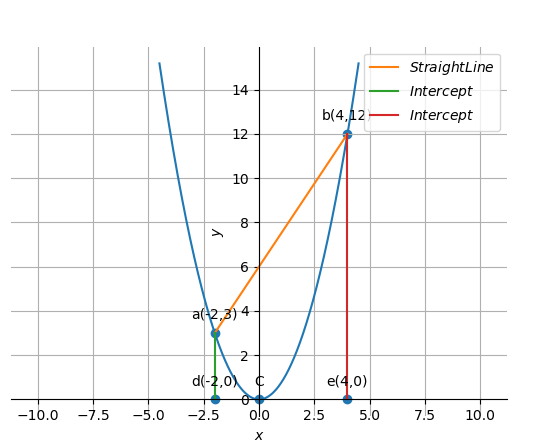
\includegraphics[width=\columnwidth]{chapters/12/8/3/7/figs/conic.png}
		\caption{}
		\label{fig:12/8/3/7}
  	\end{figure}
\iffalse
\vspace{5mm}
%-----------------------------solution---------------------------
\raggedright \textbf{SOLUTION}:\vspace{2mm}\\

%---------given----------------%
\raggedright \textbf{Given}:\vspace{2mm}\\
Equation of parabola is \\\vspace{1mm}
\begin{align}
4y=3x^2
\end{align}
Equation of line is \\ \vspace{1mm}
\begin{align}
2y=3x+12
\end{align}
%-------------To find ------------------%
\textbf{To Find }\vspace{2mm}\\
To find the intersection points and area enclosed by the parabola and line shown in figure\vspace{2mm}  \\ 
%--------------steps----------------------%
\textbf{STEP-1}\vspace{2mm}\\
The given parabola can be expressed as conics with parameters,\\ \vspace{1mm}
\begin{align}
	\vec{x}^{\top}\vec{V}\vec{x} + 2\vec{u}^{\top} \vec{x} + f = 0
\end{align}
\fi
The parameters of the given conic are
\begin{align}
\vec{V}=\myvec{
3 & 0\\
0 & 0
},
\vec{u}=\myvec{0\\-2},
f=0.
\end{align} 
For the line, the parameters are
\iffalse
\textbf{STEP-2}\vspace{2mm}\\
the given line equation can be written as\\ 
\begin{align} 
	\vec{n}^{\top}\vec{X}=c
\end{align}
Where
\begin{align}
\vec{n}=\myvec{-3\\2},\vec{m}=\myvec{2\\3}
\end{align}
\textbf{STEP-3}\vspace{2mm}\\
The points of intersection of the line, \\ 
\begin{align}
L: \quad \vec{x} = \vec{q} + \kappa \vec{m} \quad \kappa \in \mathbb{R}
\end{align}
with the conic section, \\ 
\begin{align}
	\vec{x}^{\top}\vec{V}\vec{x} + 2\vec{u}^{\top} \vec{x} + f = 0
\end{align}
are given by \\
\begin{align}
\vec{x}_i = \vec{q} + \kappa_i \vec{m}
\end{align}
where, \\
{\tiny
\begin{multline}
\kappa_i = \frac{1}
{
\vec{m}^T\vec{V}\vec{m}
}
\lbrak{-\vec{m}^T\brak{\vec{V}\vec{q}+\vec{u}}}
\\
\pm
\rbrak{\sqrt{
\sbrak{
\vec{m}^T\brak{\vec{V}\vec{q}+\vec{u}}
}^2
-
\brak
{
\vec{q}^T\vec{V}\vec{q} + 2\vec{u}^T\vec{q} +f
}
\brak{\vec{m}^T\vec{V}\vec{m}}
}
}
\end{multline}
}
On substituting\\
\fi
\begin{align}
\vec{h} = \myvec{
-2\\
3
},
\vec{m} = \myvec{2 \\ 3}
\end{align}
\iffalse
With the given parabola as in eq(3),(4),(5),\\ 

The value of $\kappa$ ,\\
\fi
yielding
\begin{align}
    \mu=-2.5,2.7
\end{align}
upon substitution in \eqref{eq:tangent_roots}
resulting in the points of intersection
\iffalse
by substituting eq(13) in eq(6)we get the
points of intersection of line with parabola \\
\fi
\begin{align}
    \vec{A}=\myvec{
-2\\
3
    },
    \vec{B}=\myvec{
4\\
12
    }.
\end{align}
From Fig. 
		\ref{fig:12/8/3/7},
		\iffalse
\textbf{Result}
\begin{center}
 \includegraphics[scale=0.5]{conic.png}    
 \end{center}\vspace{1mm}
 From the figure,\\ \vspace{1mm}
Total area of portion is given by, \\ \vspace{1mm}
Total Area=(area enclosed by the line)-(area of parabola under the line )

\subsection*{Area Under the line}
\fi
the desired area is 
\begin{align}
\int_{-2}^{4} \frac{3x+12}{2} \,dx
-\int_{-2}^{4}\frac{3x^2}{4} \,dx 
= 27 
\end{align}
\iffalse
 \vspace{2mm} \textbf{Construction}
\begin{center}
\setlength{\arrayrulewidth}{0.5mm}
\setlength{\tabcolsep}{6pt}
\renewcommand{\arraystretch}{1.5}
    \begin{tabular}{|l|c|}
    \hline 
    \textbf{Points} & \textbf{coordinates} \\ \hline
   B & $\myvec{
   4\\
   12
   } $ \\\hline
   A & $\myvec{
   -2\\
   3
   } $ \\\hline
      \end{tabular}
  \end{center}
  \end{multicols}
 
Get the python code of the figures from

\begin{table}[h]
\large
\centering
\framebox{
\url{https://github.com/chandana531/cchandana_fwc/blob/main/conic_assignment/code/conic.py}}
\bibliographystyle{ieeetr}
\end{table} 
 
\end{document}
 
\fi

\item 
\label{chapters/12/8/3/7}
\iffalse
\documentclass[10pt,a4paper]{report}
%\usepackage[latin1]{inputenc}
\usepackage[utf8]{inputenc}
\usepackage{amsmath}
\usepackage{amsfonts}
\usepackage{amssymb}
\usepackage{graphicx}
\usepackage{multicol}
\usepackage{tabularx}
\usepackage{tikz}
\usetikzlibrary{arrows,shapes,automata,petri,positioning,calc}
\usepackage{hyperref}
\usepackage{tikz}
\usetikzlibrary{matrix,calc}
\usepackage[margin=0.5in]{geometry}
% ---- power functions -----% 
\newcommand{\myvec}[1]{\ensuremath{\begin{pmatrix}#1\end{pmatrix}}}
\let\vec\mathbf

\providecommand{\norm}[1]{\left\lVert#1\right\rVert}
\providecommand{\abs}[1]{\left\vert#1\right\vert}
\let\vec\mathbf

\newcommand{\mydet}[1]{\ensuremath{\begin{vmatrix}#1\end{vmatrix}}}
\providecommand{\brak}[1]{\ensuremath{\left(#1\right)}}
\providecommand{\lbrak}[1]{\ensuremath{\left(#1\right.}}
\providecommand{\rbrak}[1]{\ensuremath{\left.#1\right)}}
\providecommand{\sbrak}[1]{\ensuremath{{}\left[#1\right]}}
%-------end power functions----%
\newenvironment{Figure}
  {\par\medskip\noindent\minipage{\linewidth}}
  {\endminipage\par\medskip}
\begin{document}
%--------------------logo figure-------------------------%
\begin{figure*}[!tbp]
  \centering
  \begin{minipage}[b]{0.4\textwidth}
    
\includegraphics[scale=0.05]{iitlogo.jpg} 
  \end{minipage}
  \hfill
  \vspace{5mm}\begin{minipage}[b]{0.4\textwidth}
\raggedleft  
\includegraphics[scale=0.05]{nrc.png}  \

  \end{minipage}\vspace{0.2cm}
\end{figure*}
%--------------------name & rollno-----------------------
\raggedright \textbf{Name}:\hspace{1mm} Cheenepalli Chandana\hspace{2cm} \Large \textbf{Conic Assignment}\hspace{2.5cm} % 
\normalsize \textbf{Roll No.} :\hspace{1mm} FWC22062\vspace{1cm}
\begin{multicols}{2}

%----------------problem statement--------------%
\raggedright \textbf{Problem Statement:}\vspace{2mm}
\raggedright \\
\fi
	Find the area enclosed by the parabola $4y=3x^2 $ and the line $2y=3x+12$.\\
	\solution
	\begin{figure}[!h]
		\centering
 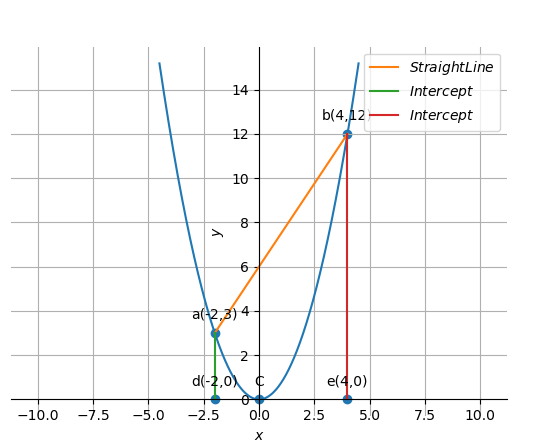
\includegraphics[width=\columnwidth]{chapters/12/8/3/7/figs/conic.png}
		\caption{}
		\label{fig:12/8/3/7}
  	\end{figure}
\iffalse
\vspace{5mm}
%-----------------------------solution---------------------------
\raggedright \textbf{SOLUTION}:\vspace{2mm}\\

%---------given----------------%
\raggedright \textbf{Given}:\vspace{2mm}\\
Equation of parabola is \\\vspace{1mm}
\begin{align}
4y=3x^2
\end{align}
Equation of line is \\ \vspace{1mm}
\begin{align}
2y=3x+12
\end{align}
%-------------To find ------------------%
\textbf{To Find }\vspace{2mm}\\
To find the intersection points and area enclosed by the parabola and line shown in figure\vspace{2mm}  \\ 
%--------------steps----------------------%
\textbf{STEP-1}\vspace{2mm}\\
The given parabola can be expressed as conics with parameters,\\ \vspace{1mm}
\begin{align}
	\vec{x}^{\top}\vec{V}\vec{x} + 2\vec{u}^{\top} \vec{x} + f = 0
\end{align}
\fi
The parameters of the given conic are
\begin{align}
\vec{V}=\myvec{
3 & 0\\
0 & 0
},
\vec{u}=\myvec{0\\-2},
f=0.
\end{align} 
For the line, the parameters are
\iffalse
\textbf{STEP-2}\vspace{2mm}\\
the given line equation can be written as\\ 
\begin{align} 
	\vec{n}^{\top}\vec{X}=c
\end{align}
Where
\begin{align}
\vec{n}=\myvec{-3\\2},\vec{m}=\myvec{2\\3}
\end{align}
\textbf{STEP-3}\vspace{2mm}\\
The points of intersection of the line, \\ 
\begin{align}
L: \quad \vec{x} = \vec{q} + \kappa \vec{m} \quad \kappa \in \mathbb{R}
\end{align}
with the conic section, \\ 
\begin{align}
	\vec{x}^{\top}\vec{V}\vec{x} + 2\vec{u}^{\top} \vec{x} + f = 0
\end{align}
are given by \\
\begin{align}
\vec{x}_i = \vec{q} + \kappa_i \vec{m}
\end{align}
where, \\
{\tiny
\begin{multline}
\kappa_i = \frac{1}
{
\vec{m}^T\vec{V}\vec{m}
}
\lbrak{-\vec{m}^T\brak{\vec{V}\vec{q}+\vec{u}}}
\\
\pm
\rbrak{\sqrt{
\sbrak{
\vec{m}^T\brak{\vec{V}\vec{q}+\vec{u}}
}^2
-
\brak
{
\vec{q}^T\vec{V}\vec{q} + 2\vec{u}^T\vec{q} +f
}
\brak{\vec{m}^T\vec{V}\vec{m}}
}
}
\end{multline}
}
On substituting\\
\fi
\begin{align}
\vec{h} = \myvec{
-2\\
3
},
\vec{m} = \myvec{2 \\ 3}
\end{align}
\iffalse
With the given parabola as in eq(3),(4),(5),\\ 

The value of $\kappa$ ,\\
\fi
yielding
\begin{align}
    \mu=-2.5,2.7
\end{align}
upon substitution in \eqref{eq:tangent_roots}
resulting in the points of intersection
\iffalse
by substituting eq(13) in eq(6)we get the
points of intersection of line with parabola \\
\fi
\begin{align}
    \vec{A}=\myvec{
-2\\
3
    },
    \vec{B}=\myvec{
4\\
12
    }.
\end{align}
From Fig. 
		\ref{fig:12/8/3/7},
		\iffalse
\textbf{Result}
\begin{center}
 \includegraphics[scale=0.5]{conic.png}    
 \end{center}\vspace{1mm}
 From the figure,\\ \vspace{1mm}
Total area of portion is given by, \\ \vspace{1mm}
Total Area=(area enclosed by the line)-(area of parabola under the line )

\subsection*{Area Under the line}
\fi
the desired area is 
\begin{align}
\int_{-2}^{4} \frac{3x+12}{2} \,dx
-\int_{-2}^{4}\frac{3x^2}{4} \,dx 
= 27 
\end{align}
\iffalse
 \vspace{2mm} \textbf{Construction}
\begin{center}
\setlength{\arrayrulewidth}{0.5mm}
\setlength{\tabcolsep}{6pt}
\renewcommand{\arraystretch}{1.5}
    \begin{tabular}{|l|c|}
    \hline 
    \textbf{Points} & \textbf{coordinates} \\ \hline
   B & $\myvec{
   4\\
   12
   } $ \\\hline
   A & $\myvec{
   -2\\
   3
   } $ \\\hline
      \end{tabular}
  \end{center}
  \end{multicols}
 
Get the python code of the figures from

\begin{table}[h]
\large
\centering
\framebox{
\url{https://github.com/chandana531/cchandana_fwc/blob/main/conic_assignment/code/conic.py}}
\bibliographystyle{ieeetr}
\end{table} 
 
\end{document}
 
\fi

\item 
\label{chapters/12/8/3/7}
\iffalse
\documentclass[10pt,a4paper]{report}
%\usepackage[latin1]{inputenc}
\usepackage[utf8]{inputenc}
\usepackage{amsmath}
\usepackage{amsfonts}
\usepackage{amssymb}
\usepackage{graphicx}
\usepackage{multicol}
\usepackage{tabularx}
\usepackage{tikz}
\usetikzlibrary{arrows,shapes,automata,petri,positioning,calc}
\usepackage{hyperref}
\usepackage{tikz}
\usetikzlibrary{matrix,calc}
\usepackage[margin=0.5in]{geometry}
% ---- power functions -----% 
\newcommand{\myvec}[1]{\ensuremath{\begin{pmatrix}#1\end{pmatrix}}}
\let\vec\mathbf

\providecommand{\norm}[1]{\left\lVert#1\right\rVert}
\providecommand{\abs}[1]{\left\vert#1\right\vert}
\let\vec\mathbf

\newcommand{\mydet}[1]{\ensuremath{\begin{vmatrix}#1\end{vmatrix}}}
\providecommand{\brak}[1]{\ensuremath{\left(#1\right)}}
\providecommand{\lbrak}[1]{\ensuremath{\left(#1\right.}}
\providecommand{\rbrak}[1]{\ensuremath{\left.#1\right)}}
\providecommand{\sbrak}[1]{\ensuremath{{}\left[#1\right]}}
%-------end power functions----%
\newenvironment{Figure}
  {\par\medskip\noindent\minipage{\linewidth}}
  {\endminipage\par\medskip}
\begin{document}
%--------------------logo figure-------------------------%
\begin{figure*}[!tbp]
  \centering
  \begin{minipage}[b]{0.4\textwidth}
    
\includegraphics[scale=0.05]{iitlogo.jpg} 
  \end{minipage}
  \hfill
  \vspace{5mm}\begin{minipage}[b]{0.4\textwidth}
\raggedleft  
\includegraphics[scale=0.05]{nrc.png}  \

  \end{minipage}\vspace{0.2cm}
\end{figure*}
%--------------------name & rollno-----------------------
\raggedright \textbf{Name}:\hspace{1mm} Cheenepalli Chandana\hspace{2cm} \Large \textbf{Conic Assignment}\hspace{2.5cm} % 
\normalsize \textbf{Roll No.} :\hspace{1mm} FWC22062\vspace{1cm}
\begin{multicols}{2}

%----------------problem statement--------------%
\raggedright \textbf{Problem Statement:}\vspace{2mm}
\raggedright \\
\fi
	Find the area enclosed by the parabola $4y=3x^2 $ and the line $2y=3x+12$.\\
	\solution
	\begin{figure}[!h]
		\centering
 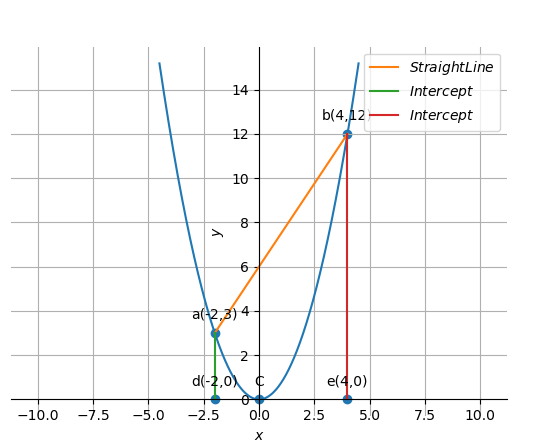
\includegraphics[width=\columnwidth]{chapters/12/8/3/7/figs/conic.png}
		\caption{}
		\label{fig:12/8/3/7}
  	\end{figure}
\iffalse
\vspace{5mm}
%-----------------------------solution---------------------------
\raggedright \textbf{SOLUTION}:\vspace{2mm}\\

%---------given----------------%
\raggedright \textbf{Given}:\vspace{2mm}\\
Equation of parabola is \\\vspace{1mm}
\begin{align}
4y=3x^2
\end{align}
Equation of line is \\ \vspace{1mm}
\begin{align}
2y=3x+12
\end{align}
%-------------To find ------------------%
\textbf{To Find }\vspace{2mm}\\
To find the intersection points and area enclosed by the parabola and line shown in figure\vspace{2mm}  \\ 
%--------------steps----------------------%
\textbf{STEP-1}\vspace{2mm}\\
The given parabola can be expressed as conics with parameters,\\ \vspace{1mm}
\begin{align}
	\vec{x}^{\top}\vec{V}\vec{x} + 2\vec{u}^{\top} \vec{x} + f = 0
\end{align}
\fi
The parameters of the given conic are
\begin{align}
\vec{V}=\myvec{
3 & 0\\
0 & 0
},
\vec{u}=\myvec{0\\-2},
f=0.
\end{align} 
For the line, the parameters are
\iffalse
\textbf{STEP-2}\vspace{2mm}\\
the given line equation can be written as\\ 
\begin{align} 
	\vec{n}^{\top}\vec{X}=c
\end{align}
Where
\begin{align}
\vec{n}=\myvec{-3\\2},\vec{m}=\myvec{2\\3}
\end{align}
\textbf{STEP-3}\vspace{2mm}\\
The points of intersection of the line, \\ 
\begin{align}
L: \quad \vec{x} = \vec{q} + \kappa \vec{m} \quad \kappa \in \mathbb{R}
\end{align}
with the conic section, \\ 
\begin{align}
	\vec{x}^{\top}\vec{V}\vec{x} + 2\vec{u}^{\top} \vec{x} + f = 0
\end{align}
are given by \\
\begin{align}
\vec{x}_i = \vec{q} + \kappa_i \vec{m}
\end{align}
where, \\
{\tiny
\begin{multline}
\kappa_i = \frac{1}
{
\vec{m}^T\vec{V}\vec{m}
}
\lbrak{-\vec{m}^T\brak{\vec{V}\vec{q}+\vec{u}}}
\\
\pm
\rbrak{\sqrt{
\sbrak{
\vec{m}^T\brak{\vec{V}\vec{q}+\vec{u}}
}^2
-
\brak
{
\vec{q}^T\vec{V}\vec{q} + 2\vec{u}^T\vec{q} +f
}
\brak{\vec{m}^T\vec{V}\vec{m}}
}
}
\end{multline}
}
On substituting\\
\fi
\begin{align}
\vec{h} = \myvec{
-2\\
3
},
\vec{m} = \myvec{2 \\ 3}
\end{align}
\iffalse
With the given parabola as in eq(3),(4),(5),\\ 

The value of $\kappa$ ,\\
\fi
yielding
\begin{align}
    \mu=-2.5,2.7
\end{align}
upon substitution in \eqref{eq:tangent_roots}
resulting in the points of intersection
\iffalse
by substituting eq(13) in eq(6)we get the
points of intersection of line with parabola \\
\fi
\begin{align}
    \vec{A}=\myvec{
-2\\
3
    },
    \vec{B}=\myvec{
4\\
12
    }.
\end{align}
From Fig. 
		\ref{fig:12/8/3/7},
		\iffalse
\textbf{Result}
\begin{center}
 \includegraphics[scale=0.5]{conic.png}    
 \end{center}\vspace{1mm}
 From the figure,\\ \vspace{1mm}
Total area of portion is given by, \\ \vspace{1mm}
Total Area=(area enclosed by the line)-(area of parabola under the line )

\subsection*{Area Under the line}
\fi
the desired area is 
\begin{align}
\int_{-2}^{4} \frac{3x+12}{2} \,dx
-\int_{-2}^{4}\frac{3x^2}{4} \,dx 
= 27 
\end{align}
\iffalse
 \vspace{2mm} \textbf{Construction}
\begin{center}
\setlength{\arrayrulewidth}{0.5mm}
\setlength{\tabcolsep}{6pt}
\renewcommand{\arraystretch}{1.5}
    \begin{tabular}{|l|c|}
    \hline 
    \textbf{Points} & \textbf{coordinates} \\ \hline
   B & $\myvec{
   4\\
   12
   } $ \\\hline
   A & $\myvec{
   -2\\
   3
   } $ \\\hline
      \end{tabular}
  \end{center}
  \end{multicols}
 
Get the python code of the figures from

\begin{table}[h]
\large
\centering
\framebox{
\url{https://github.com/chandana531/cchandana_fwc/blob/main/conic_assignment/code/conic.py}}
\bibliographystyle{ieeetr}
\end{table} 
 
\end{document}
 
\fi

\item 
\label{chapters/12/8/3/7}
\iffalse
\documentclass[10pt,a4paper]{report}
%\usepackage[latin1]{inputenc}
\usepackage[utf8]{inputenc}
\usepackage{amsmath}
\usepackage{amsfonts}
\usepackage{amssymb}
\usepackage{graphicx}
\usepackage{multicol}
\usepackage{tabularx}
\usepackage{tikz}
\usetikzlibrary{arrows,shapes,automata,petri,positioning,calc}
\usepackage{hyperref}
\usepackage{tikz}
\usetikzlibrary{matrix,calc}
\usepackage[margin=0.5in]{geometry}
% ---- power functions -----% 
\newcommand{\myvec}[1]{\ensuremath{\begin{pmatrix}#1\end{pmatrix}}}
\let\vec\mathbf

\providecommand{\norm}[1]{\left\lVert#1\right\rVert}
\providecommand{\abs}[1]{\left\vert#1\right\vert}
\let\vec\mathbf

\newcommand{\mydet}[1]{\ensuremath{\begin{vmatrix}#1\end{vmatrix}}}
\providecommand{\brak}[1]{\ensuremath{\left(#1\right)}}
\providecommand{\lbrak}[1]{\ensuremath{\left(#1\right.}}
\providecommand{\rbrak}[1]{\ensuremath{\left.#1\right)}}
\providecommand{\sbrak}[1]{\ensuremath{{}\left[#1\right]}}
%-------end power functions----%
\newenvironment{Figure}
  {\par\medskip\noindent\minipage{\linewidth}}
  {\endminipage\par\medskip}
\begin{document}
%--------------------logo figure-------------------------%
\begin{figure*}[!tbp]
  \centering
  \begin{minipage}[b]{0.4\textwidth}
    
\includegraphics[scale=0.05]{iitlogo.jpg} 
  \end{minipage}
  \hfill
  \vspace{5mm}\begin{minipage}[b]{0.4\textwidth}
\raggedleft  
\includegraphics[scale=0.05]{nrc.png}  \

  \end{minipage}\vspace{0.2cm}
\end{figure*}
%--------------------name & rollno-----------------------
\raggedright \textbf{Name}:\hspace{1mm} Cheenepalli Chandana\hspace{2cm} \Large \textbf{Conic Assignment}\hspace{2.5cm} % 
\normalsize \textbf{Roll No.} :\hspace{1mm} FWC22062\vspace{1cm}
\begin{multicols}{2}

%----------------problem statement--------------%
\raggedright \textbf{Problem Statement:}\vspace{2mm}
\raggedright \\
\fi
	Find the area enclosed by the parabola $4y=3x^2 $ and the line $2y=3x+12$.\\
	\solution
	\begin{figure}[!h]
		\centering
 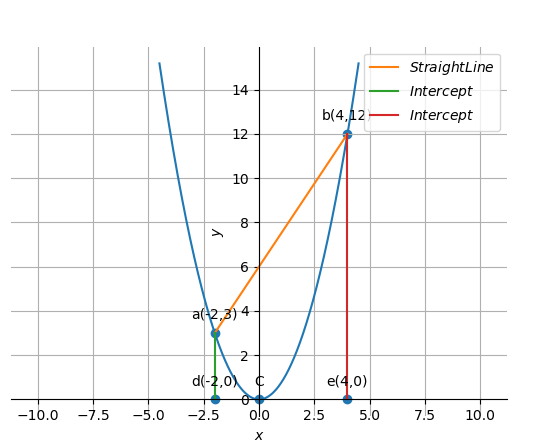
\includegraphics[width=\columnwidth]{chapters/12/8/3/7/figs/conic.png}
		\caption{}
		\label{fig:12/8/3/7}
  	\end{figure}
\iffalse
\vspace{5mm}
%-----------------------------solution---------------------------
\raggedright \textbf{SOLUTION}:\vspace{2mm}\\

%---------given----------------%
\raggedright \textbf{Given}:\vspace{2mm}\\
Equation of parabola is \\\vspace{1mm}
\begin{align}
4y=3x^2
\end{align}
Equation of line is \\ \vspace{1mm}
\begin{align}
2y=3x+12
\end{align}
%-------------To find ------------------%
\textbf{To Find }\vspace{2mm}\\
To find the intersection points and area enclosed by the parabola and line shown in figure\vspace{2mm}  \\ 
%--------------steps----------------------%
\textbf{STEP-1}\vspace{2mm}\\
The given parabola can be expressed as conics with parameters,\\ \vspace{1mm}
\begin{align}
	\vec{x}^{\top}\vec{V}\vec{x} + 2\vec{u}^{\top} \vec{x} + f = 0
\end{align}
\fi
The parameters of the given conic are
\begin{align}
\vec{V}=\myvec{
3 & 0\\
0 & 0
},
\vec{u}=\myvec{0\\-2},
f=0.
\end{align} 
For the line, the parameters are
\iffalse
\textbf{STEP-2}\vspace{2mm}\\
the given line equation can be written as\\ 
\begin{align} 
	\vec{n}^{\top}\vec{X}=c
\end{align}
Where
\begin{align}
\vec{n}=\myvec{-3\\2},\vec{m}=\myvec{2\\3}
\end{align}
\textbf{STEP-3}\vspace{2mm}\\
The points of intersection of the line, \\ 
\begin{align}
L: \quad \vec{x} = \vec{q} + \kappa \vec{m} \quad \kappa \in \mathbb{R}
\end{align}
with the conic section, \\ 
\begin{align}
	\vec{x}^{\top}\vec{V}\vec{x} + 2\vec{u}^{\top} \vec{x} + f = 0
\end{align}
are given by \\
\begin{align}
\vec{x}_i = \vec{q} + \kappa_i \vec{m}
\end{align}
where, \\
{\tiny
\begin{multline}
\kappa_i = \frac{1}
{
\vec{m}^T\vec{V}\vec{m}
}
\lbrak{-\vec{m}^T\brak{\vec{V}\vec{q}+\vec{u}}}
\\
\pm
\rbrak{\sqrt{
\sbrak{
\vec{m}^T\brak{\vec{V}\vec{q}+\vec{u}}
}^2
-
\brak
{
\vec{q}^T\vec{V}\vec{q} + 2\vec{u}^T\vec{q} +f
}
\brak{\vec{m}^T\vec{V}\vec{m}}
}
}
\end{multline}
}
On substituting\\
\fi
\begin{align}
\vec{h} = \myvec{
-2\\
3
},
\vec{m} = \myvec{2 \\ 3}
\end{align}
\iffalse
With the given parabola as in eq(3),(4),(5),\\ 

The value of $\kappa$ ,\\
\fi
yielding
\begin{align}
    \mu=-2.5,2.7
\end{align}
upon substitution in \eqref{eq:tangent_roots}
resulting in the points of intersection
\iffalse
by substituting eq(13) in eq(6)we get the
points of intersection of line with parabola \\
\fi
\begin{align}
    \vec{A}=\myvec{
-2\\
3
    },
    \vec{B}=\myvec{
4\\
12
    }.
\end{align}
From Fig. 
		\ref{fig:12/8/3/7},
		\iffalse
\textbf{Result}
\begin{center}
 \includegraphics[scale=0.5]{conic.png}    
 \end{center}\vspace{1mm}
 From the figure,\\ \vspace{1mm}
Total area of portion is given by, \\ \vspace{1mm}
Total Area=(area enclosed by the line)-(area of parabola under the line )

\subsection*{Area Under the line}
\fi
the desired area is 
\begin{align}
\int_{-2}^{4} \frac{3x+12}{2} \,dx
-\int_{-2}^{4}\frac{3x^2}{4} \,dx 
= 27 
\end{align}
\iffalse
 \vspace{2mm} \textbf{Construction}
\begin{center}
\setlength{\arrayrulewidth}{0.5mm}
\setlength{\tabcolsep}{6pt}
\renewcommand{\arraystretch}{1.5}
    \begin{tabular}{|l|c|}
    \hline 
    \textbf{Points} & \textbf{coordinates} \\ \hline
   B & $\myvec{
   4\\
   12
   } $ \\\hline
   A & $\myvec{
   -2\\
   3
   } $ \\\hline
      \end{tabular}
  \end{center}
  \end{multicols}
 
Get the python code of the figures from

\begin{table}[h]
\large
\centering
\framebox{
\url{https://github.com/chandana531/cchandana_fwc/blob/main/conic_assignment/code/conic.py}}
\bibliographystyle{ieeetr}
\end{table} 
 
\end{document}
 
\fi

\item 
\label{chapters/12/8/3/7}
\iffalse
\documentclass[10pt,a4paper]{report}
%\usepackage[latin1]{inputenc}
\usepackage[utf8]{inputenc}
\usepackage{amsmath}
\usepackage{amsfonts}
\usepackage{amssymb}
\usepackage{graphicx}
\usepackage{multicol}
\usepackage{tabularx}
\usepackage{tikz}
\usetikzlibrary{arrows,shapes,automata,petri,positioning,calc}
\usepackage{hyperref}
\usepackage{tikz}
\usetikzlibrary{matrix,calc}
\usepackage[margin=0.5in]{geometry}
% ---- power functions -----% 
\newcommand{\myvec}[1]{\ensuremath{\begin{pmatrix}#1\end{pmatrix}}}
\let\vec\mathbf

\providecommand{\norm}[1]{\left\lVert#1\right\rVert}
\providecommand{\abs}[1]{\left\vert#1\right\vert}
\let\vec\mathbf

\newcommand{\mydet}[1]{\ensuremath{\begin{vmatrix}#1\end{vmatrix}}}
\providecommand{\brak}[1]{\ensuremath{\left(#1\right)}}
\providecommand{\lbrak}[1]{\ensuremath{\left(#1\right.}}
\providecommand{\rbrak}[1]{\ensuremath{\left.#1\right)}}
\providecommand{\sbrak}[1]{\ensuremath{{}\left[#1\right]}}
%-------end power functions----%
\newenvironment{Figure}
  {\par\medskip\noindent\minipage{\linewidth}}
  {\endminipage\par\medskip}
\begin{document}
%--------------------logo figure-------------------------%
\begin{figure*}[!tbp]
  \centering
  \begin{minipage}[b]{0.4\textwidth}
    
\includegraphics[scale=0.05]{iitlogo.jpg} 
  \end{minipage}
  \hfill
  \vspace{5mm}\begin{minipage}[b]{0.4\textwidth}
\raggedleft  
\includegraphics[scale=0.05]{nrc.png}  \

  \end{minipage}\vspace{0.2cm}
\end{figure*}
%--------------------name & rollno-----------------------
\raggedright \textbf{Name}:\hspace{1mm} Cheenepalli Chandana\hspace{2cm} \Large \textbf{Conic Assignment}\hspace{2.5cm} % 
\normalsize \textbf{Roll No.} :\hspace{1mm} FWC22062\vspace{1cm}
\begin{multicols}{2}

%----------------problem statement--------------%
\raggedright \textbf{Problem Statement:}\vspace{2mm}
\raggedright \\
\fi
	Find the area enclosed by the parabola $4y=3x^2 $ and the line $2y=3x+12$.\\
	\solution
	\begin{figure}[!h]
		\centering
 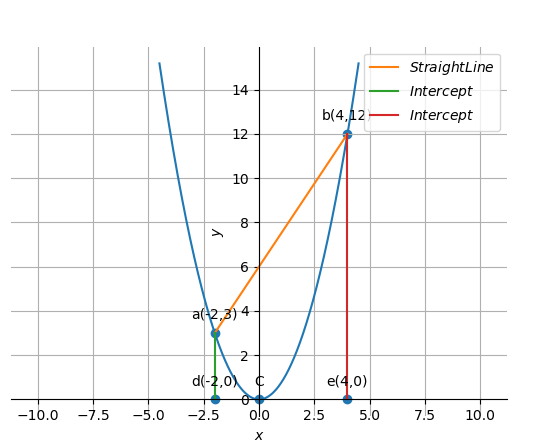
\includegraphics[width=\columnwidth]{chapters/12/8/3/7/figs/conic.png}
		\caption{}
		\label{fig:12/8/3/7}
  	\end{figure}
\iffalse
\vspace{5mm}
%-----------------------------solution---------------------------
\raggedright \textbf{SOLUTION}:\vspace{2mm}\\

%---------given----------------%
\raggedright \textbf{Given}:\vspace{2mm}\\
Equation of parabola is \\\vspace{1mm}
\begin{align}
4y=3x^2
\end{align}
Equation of line is \\ \vspace{1mm}
\begin{align}
2y=3x+12
\end{align}
%-------------To find ------------------%
\textbf{To Find }\vspace{2mm}\\
To find the intersection points and area enclosed by the parabola and line shown in figure\vspace{2mm}  \\ 
%--------------steps----------------------%
\textbf{STEP-1}\vspace{2mm}\\
The given parabola can be expressed as conics with parameters,\\ \vspace{1mm}
\begin{align}
	\vec{x}^{\top}\vec{V}\vec{x} + 2\vec{u}^{\top} \vec{x} + f = 0
\end{align}
\fi
The parameters of the given conic are
\begin{align}
\vec{V}=\myvec{
3 & 0\\
0 & 0
},
\vec{u}=\myvec{0\\-2},
f=0.
\end{align} 
For the line, the parameters are
\iffalse
\textbf{STEP-2}\vspace{2mm}\\
the given line equation can be written as\\ 
\begin{align} 
	\vec{n}^{\top}\vec{X}=c
\end{align}
Where
\begin{align}
\vec{n}=\myvec{-3\\2},\vec{m}=\myvec{2\\3}
\end{align}
\textbf{STEP-3}\vspace{2mm}\\
The points of intersection of the line, \\ 
\begin{align}
L: \quad \vec{x} = \vec{q} + \kappa \vec{m} \quad \kappa \in \mathbb{R}
\end{align}
with the conic section, \\ 
\begin{align}
	\vec{x}^{\top}\vec{V}\vec{x} + 2\vec{u}^{\top} \vec{x} + f = 0
\end{align}
are given by \\
\begin{align}
\vec{x}_i = \vec{q} + \kappa_i \vec{m}
\end{align}
where, \\
{\tiny
\begin{multline}
\kappa_i = \frac{1}
{
\vec{m}^T\vec{V}\vec{m}
}
\lbrak{-\vec{m}^T\brak{\vec{V}\vec{q}+\vec{u}}}
\\
\pm
\rbrak{\sqrt{
\sbrak{
\vec{m}^T\brak{\vec{V}\vec{q}+\vec{u}}
}^2
-
\brak
{
\vec{q}^T\vec{V}\vec{q} + 2\vec{u}^T\vec{q} +f
}
\brak{\vec{m}^T\vec{V}\vec{m}}
}
}
\end{multline}
}
On substituting\\
\fi
\begin{align}
\vec{h} = \myvec{
-2\\
3
},
\vec{m} = \myvec{2 \\ 3}
\end{align}
\iffalse
With the given parabola as in eq(3),(4),(5),\\ 

The value of $\kappa$ ,\\
\fi
yielding
\begin{align}
    \mu=-2.5,2.7
\end{align}
upon substitution in \eqref{eq:tangent_roots}
resulting in the points of intersection
\iffalse
by substituting eq(13) in eq(6)we get the
points of intersection of line with parabola \\
\fi
\begin{align}
    \vec{A}=\myvec{
-2\\
3
    },
    \vec{B}=\myvec{
4\\
12
    }.
\end{align}
From Fig. 
		\ref{fig:12/8/3/7},
		\iffalse
\textbf{Result}
\begin{center}
 \includegraphics[scale=0.5]{conic.png}    
 \end{center}\vspace{1mm}
 From the figure,\\ \vspace{1mm}
Total area of portion is given by, \\ \vspace{1mm}
Total Area=(area enclosed by the line)-(area of parabola under the line )

\subsection*{Area Under the line}
\fi
the desired area is 
\begin{align}
\int_{-2}^{4} \frac{3x+12}{2} \,dx
-\int_{-2}^{4}\frac{3x^2}{4} \,dx 
= 27 
\end{align}
\iffalse
 \vspace{2mm} \textbf{Construction}
\begin{center}
\setlength{\arrayrulewidth}{0.5mm}
\setlength{\tabcolsep}{6pt}
\renewcommand{\arraystretch}{1.5}
    \begin{tabular}{|l|c|}
    \hline 
    \textbf{Points} & \textbf{coordinates} \\ \hline
   B & $\myvec{
   4\\
   12
   } $ \\\hline
   A & $\myvec{
   -2\\
   3
   } $ \\\hline
      \end{tabular}
  \end{center}
  \end{multicols}
 
Get the python code of the figures from

\begin{table}[h]
\large
\centering
\framebox{
\url{https://github.com/chandana531/cchandana_fwc/blob/main/conic_assignment/code/conic.py}}
\bibliographystyle{ieeetr}
\end{table} 
 
\end{document}
 
\fi

\item 
\label{chapters/12/8/3/7}
\iffalse
\documentclass[10pt,a4paper]{report}
%\usepackage[latin1]{inputenc}
\usepackage[utf8]{inputenc}
\usepackage{amsmath}
\usepackage{amsfonts}
\usepackage{amssymb}
\usepackage{graphicx}
\usepackage{multicol}
\usepackage{tabularx}
\usepackage{tikz}
\usetikzlibrary{arrows,shapes,automata,petri,positioning,calc}
\usepackage{hyperref}
\usepackage{tikz}
\usetikzlibrary{matrix,calc}
\usepackage[margin=0.5in]{geometry}
% ---- power functions -----% 
\newcommand{\myvec}[1]{\ensuremath{\begin{pmatrix}#1\end{pmatrix}}}
\let\vec\mathbf

\providecommand{\norm}[1]{\left\lVert#1\right\rVert}
\providecommand{\abs}[1]{\left\vert#1\right\vert}
\let\vec\mathbf

\newcommand{\mydet}[1]{\ensuremath{\begin{vmatrix}#1\end{vmatrix}}}
\providecommand{\brak}[1]{\ensuremath{\left(#1\right)}}
\providecommand{\lbrak}[1]{\ensuremath{\left(#1\right.}}
\providecommand{\rbrak}[1]{\ensuremath{\left.#1\right)}}
\providecommand{\sbrak}[1]{\ensuremath{{}\left[#1\right]}}
%-------end power functions----%
\newenvironment{Figure}
  {\par\medskip\noindent\minipage{\linewidth}}
  {\endminipage\par\medskip}
\begin{document}
%--------------------logo figure-------------------------%
\begin{figure*}[!tbp]
  \centering
  \begin{minipage}[b]{0.4\textwidth}
    
\includegraphics[scale=0.05]{iitlogo.jpg} 
  \end{minipage}
  \hfill
  \vspace{5mm}\begin{minipage}[b]{0.4\textwidth}
\raggedleft  
\includegraphics[scale=0.05]{nrc.png}  \

  \end{minipage}\vspace{0.2cm}
\end{figure*}
%--------------------name & rollno-----------------------
\raggedright \textbf{Name}:\hspace{1mm} Cheenepalli Chandana\hspace{2cm} \Large \textbf{Conic Assignment}\hspace{2.5cm} % 
\normalsize \textbf{Roll No.} :\hspace{1mm} FWC22062\vspace{1cm}
\begin{multicols}{2}

%----------------problem statement--------------%
\raggedright \textbf{Problem Statement:}\vspace{2mm}
\raggedright \\
\fi
	Find the area enclosed by the parabola $4y=3x^2 $ and the line $2y=3x+12$.\\
	\solution
	\begin{figure}[!h]
		\centering
 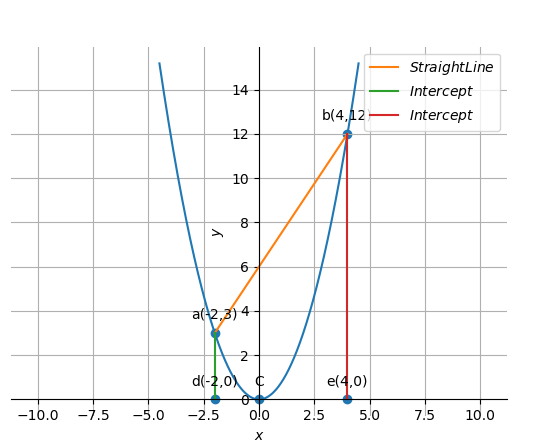
\includegraphics[width=\columnwidth]{chapters/12/8/3/7/figs/conic.png}
		\caption{}
		\label{fig:12/8/3/7}
  	\end{figure}
\iffalse
\vspace{5mm}
%-----------------------------solution---------------------------
\raggedright \textbf{SOLUTION}:\vspace{2mm}\\

%---------given----------------%
\raggedright \textbf{Given}:\vspace{2mm}\\
Equation of parabola is \\\vspace{1mm}
\begin{align}
4y=3x^2
\end{align}
Equation of line is \\ \vspace{1mm}
\begin{align}
2y=3x+12
\end{align}
%-------------To find ------------------%
\textbf{To Find }\vspace{2mm}\\
To find the intersection points and area enclosed by the parabola and line shown in figure\vspace{2mm}  \\ 
%--------------steps----------------------%
\textbf{STEP-1}\vspace{2mm}\\
The given parabola can be expressed as conics with parameters,\\ \vspace{1mm}
\begin{align}
	\vec{x}^{\top}\vec{V}\vec{x} + 2\vec{u}^{\top} \vec{x} + f = 0
\end{align}
\fi
The parameters of the given conic are
\begin{align}
\vec{V}=\myvec{
3 & 0\\
0 & 0
},
\vec{u}=\myvec{0\\-2},
f=0.
\end{align} 
For the line, the parameters are
\iffalse
\textbf{STEP-2}\vspace{2mm}\\
the given line equation can be written as\\ 
\begin{align} 
	\vec{n}^{\top}\vec{X}=c
\end{align}
Where
\begin{align}
\vec{n}=\myvec{-3\\2},\vec{m}=\myvec{2\\3}
\end{align}
\textbf{STEP-3}\vspace{2mm}\\
The points of intersection of the line, \\ 
\begin{align}
L: \quad \vec{x} = \vec{q} + \kappa \vec{m} \quad \kappa \in \mathbb{R}
\end{align}
with the conic section, \\ 
\begin{align}
	\vec{x}^{\top}\vec{V}\vec{x} + 2\vec{u}^{\top} \vec{x} + f = 0
\end{align}
are given by \\
\begin{align}
\vec{x}_i = \vec{q} + \kappa_i \vec{m}
\end{align}
where, \\
{\tiny
\begin{multline}
\kappa_i = \frac{1}
{
\vec{m}^T\vec{V}\vec{m}
}
\lbrak{-\vec{m}^T\brak{\vec{V}\vec{q}+\vec{u}}}
\\
\pm
\rbrak{\sqrt{
\sbrak{
\vec{m}^T\brak{\vec{V}\vec{q}+\vec{u}}
}^2
-
\brak
{
\vec{q}^T\vec{V}\vec{q} + 2\vec{u}^T\vec{q} +f
}
\brak{\vec{m}^T\vec{V}\vec{m}}
}
}
\end{multline}
}
On substituting\\
\fi
\begin{align}
\vec{h} = \myvec{
-2\\
3
},
\vec{m} = \myvec{2 \\ 3}
\end{align}
\iffalse
With the given parabola as in eq(3),(4),(5),\\ 

The value of $\kappa$ ,\\
\fi
yielding
\begin{align}
    \mu=-2.5,2.7
\end{align}
upon substitution in \eqref{eq:tangent_roots}
resulting in the points of intersection
\iffalse
by substituting eq(13) in eq(6)we get the
points of intersection of line with parabola \\
\fi
\begin{align}
    \vec{A}=\myvec{
-2\\
3
    },
    \vec{B}=\myvec{
4\\
12
    }.
\end{align}
From Fig. 
		\ref{fig:12/8/3/7},
		\iffalse
\textbf{Result}
\begin{center}
 \includegraphics[scale=0.5]{conic.png}    
 \end{center}\vspace{1mm}
 From the figure,\\ \vspace{1mm}
Total area of portion is given by, \\ \vspace{1mm}
Total Area=(area enclosed by the line)-(area of parabola under the line )

\subsection*{Area Under the line}
\fi
the desired area is 
\begin{align}
\int_{-2}^{4} \frac{3x+12}{2} \,dx
-\int_{-2}^{4}\frac{3x^2}{4} \,dx 
= 27 
\end{align}
\iffalse
 \vspace{2mm} \textbf{Construction}
\begin{center}
\setlength{\arrayrulewidth}{0.5mm}
\setlength{\tabcolsep}{6pt}
\renewcommand{\arraystretch}{1.5}
    \begin{tabular}{|l|c|}
    \hline 
    \textbf{Points} & \textbf{coordinates} \\ \hline
   B & $\myvec{
   4\\
   12
   } $ \\\hline
   A & $\myvec{
   -2\\
   3
   } $ \\\hline
      \end{tabular}
  \end{center}
  \end{multicols}
 
Get the python code of the figures from

\begin{table}[h]
\large
\centering
\framebox{
\url{https://github.com/chandana531/cchandana_fwc/blob/main/conic_assignment/code/conic.py}}
\bibliographystyle{ieeetr}
\end{table} 
 
\end{document}
 
\fi

\item 
\label{chapters/12/8/3/7}
\iffalse
\documentclass[10pt,a4paper]{report}
%\usepackage[latin1]{inputenc}
\usepackage[utf8]{inputenc}
\usepackage{amsmath}
\usepackage{amsfonts}
\usepackage{amssymb}
\usepackage{graphicx}
\usepackage{multicol}
\usepackage{tabularx}
\usepackage{tikz}
\usetikzlibrary{arrows,shapes,automata,petri,positioning,calc}
\usepackage{hyperref}
\usepackage{tikz}
\usetikzlibrary{matrix,calc}
\usepackage[margin=0.5in]{geometry}
% ---- power functions -----% 
\newcommand{\myvec}[1]{\ensuremath{\begin{pmatrix}#1\end{pmatrix}}}
\let\vec\mathbf

\providecommand{\norm}[1]{\left\lVert#1\right\rVert}
\providecommand{\abs}[1]{\left\vert#1\right\vert}
\let\vec\mathbf

\newcommand{\mydet}[1]{\ensuremath{\begin{vmatrix}#1\end{vmatrix}}}
\providecommand{\brak}[1]{\ensuremath{\left(#1\right)}}
\providecommand{\lbrak}[1]{\ensuremath{\left(#1\right.}}
\providecommand{\rbrak}[1]{\ensuremath{\left.#1\right)}}
\providecommand{\sbrak}[1]{\ensuremath{{}\left[#1\right]}}
%-------end power functions----%
\newenvironment{Figure}
  {\par\medskip\noindent\minipage{\linewidth}}
  {\endminipage\par\medskip}
\begin{document}
%--------------------logo figure-------------------------%
\begin{figure*}[!tbp]
  \centering
  \begin{minipage}[b]{0.4\textwidth}
    \includegraphics[scale=0.05]{iitlogo.jpg} 
  \end{minipage}
  \hfill
  \vspace{5mm}\begin{minipage}[b]{0.4\textwidth}
\raggedleft  \includegraphics[scale=0.05]{nrc.png}  \

  \end{minipage}\vspace{0.2cm}
\end{figure*}
%--------------------name & rollno-----------------------
\raggedright \textbf{Name}:\hspace{1mm} Cheenepalli Chandana\hspace{2cm} \Large \textbf{Conic Assignment}\hspace{2.5cm} % 
\normalsize \textbf{Roll No.} :\hspace{1mm} FWC22062\vspace{1cm}
\begin{multicols}{2}

%----------------problem statement--------------%
\raggedright \textbf{Problem Statement:}\vspace{2mm}
\raggedright \\
\fi
	Find the area enclosed by the parabola $4y=3x^2 $ and the line $2y=3x+12$.\\
	\solution
	\begin{figure}[!h]
		\centering
 \includegraphics[width=\columnwidth]{chapters/12/8/3/7/figs/conic.png}
		\caption{}
		\label{fig:12/8/3/7}
  	\end{figure}
\iffalse
\vspace{5mm}
%-----------------------------solution---------------------------
\raggedright \textbf{SOLUTION}:\vspace{2mm}\\

%---------given----------------%
\raggedright \textbf{Given}:\vspace{2mm}\\
Equation of parabola is \\\vspace{1mm}
\begin{align}
4y=3x^2
\end{align}
Equation of line is \\ \vspace{1mm}
\begin{align}
2y=3x+12
\end{align}
%-------------To find ------------------%
\textbf{To Find }\vspace{2mm}\\
To find the intersection points and area enclosed by the parabola and line shown in figure\vspace{2mm}  \\ 
%--------------steps----------------------%
\textbf{STEP-1}\vspace{2mm}\\
The given parabola can be expressed as conics with parameters,\\ \vspace{1mm}
\begin{align}
	\vec{x}^{\top}\vec{V}\vec{x} + 2\vec{u}^{\top} \vec{x} + f = 0
\end{align}
\fi
The parameters of the given conic are
\begin{align}
\vec{V}=\myvec{
3 & 0\\
0 & 0
},
\vec{u}=\myvec{0\\-2},
f=0.
\end{align} 
For the line, the parameters are
\iffalse
\textbf{STEP-2}\vspace{2mm}\\
the given line equation can be written as\\ 
\begin{align} 
	\vec{n}^{\top}\vec{X}=c
\end{align}
Where
\begin{align}
\vec{n}=\myvec{-3\\2},\vec{m}=\myvec{2\\3}
\end{align}
\textbf{STEP-3}\vspace{2mm}\\
The points of intersection of the line, \\ 
\begin{align}
L: \quad \vec{x} = \vec{q} + \kappa \vec{m} \quad \kappa \in \mathbb{R}
\end{align}
with the conic section, \\ 
\begin{align}
	\vec{x}^{\top}\vec{V}\vec{x} + 2\vec{u}^{\top} \vec{x} + f = 0
\end{align}
are given by \\
\begin{align}
\vec{x}_i = \vec{q} + \kappa_i \vec{m}
\end{align}
where, \\
{\tiny
\begin{multline}
\kappa_i = \frac{1}
{
\vec{m}^T\vec{V}\vec{m}
}
\lbrak{-\vec{m}^T\brak{\vec{V}\vec{q}+\vec{u}}}
\\
\pm
\rbrak{\sqrt{
\sbrak{
\vec{m}^T\brak{\vec{V}\vec{q}+\vec{u}}
}^2
-
\brak
{
\vec{q}^T\vec{V}\vec{q} + 2\vec{u}^T\vec{q} +f
}
\brak{\vec{m}^T\vec{V}\vec{m}}
}
}
\end{multline}
}
On substituting\\
\fi
\begin{align}
\vec{h} = \myvec{
-2\\
3
},
\vec{m} = \myvec{2 \\ 3}
\end{align}
\iffalse
With the given parabola as in eq(3),(4),(5),\\ 

The value of $\kappa$ ,\\
\fi
yielding
\begin{align}
    \mu=-2.5,2.7
\end{align}
upon substitution in \eqref{eq:tangent_roots}
resulting in the points of intersection
\iffalse
by substituting eq(13) in eq(6)we get the
points of intersection of line with parabola \\
\fi
\begin{align}
    \vec{A}=\myvec{
-2\\
3
    },
    \vec{B}=\myvec{
4\\
12
    }.
\end{align}
From Fig. 
		\ref{fig:12/8/3/7},
		\iffalse
\textbf{Result}
\begin{center}
 \includegraphics[scale=0.5]{conic.png}    
 \end{center}\vspace{1mm}
 From the figure,\\ \vspace{1mm}
Total area of portion is given by, \\ \vspace{1mm}
Total Area=(area enclosed by the line)-(area of parabola under the line )

\subsection*{Area Under the line}
\fi
the desired area is 
\begin{align}
\int_{-2}^{4} \frac{3x+12}{2} \,dx
-\int_{-2}^{4}\frac{3x^2}{4} \,dx 
= 27 
\end{align}
\iffalse
 \vspace{2mm} \textbf{Construction}
\begin{center}
\setlength{\arrayrulewidth}{0.5mm}
\setlength{\tabcolsep}{6pt}
\renewcommand{\arraystretch}{1.5}
    \begin{tabular}{|l|c|}
    \hline 
    \textbf{Points} & \textbf{coordinates} \\ \hline
   B & $\myvec{
   4\\
   12
   } $ \\\hline
   A & $\myvec{
   -2\\
   3
   } $ \\\hline
      \end{tabular}
  \end{center}
  \end{multicols}
 
Get the python code of the figures from

\begin{table}[h]
\large
\centering
\framebox{
\url{https://github.com/chandana531/cchandana_fwc/blob/main/conic_assignment/code/conic.py}}
\bibliographystyle{ieeetr}
\end{table} 
 
\end{document}
 
\fi

\fi
\end{enumerate}
